\documentclass[twoside]{book}

% Packages required by doxygen
\usepackage{fixltx2e}
\usepackage{calc}
\usepackage{doxygen}
\usepackage[export]{adjustbox} % also loads graphicx
\usepackage{graphicx}
\usepackage[utf8]{inputenc}
\usepackage{makeidx}
\usepackage{multicol}
\usepackage{multirow}
\PassOptionsToPackage{warn}{textcomp}
\usepackage{textcomp}
\usepackage[nointegrals]{wasysym}
\usepackage[table]{xcolor}

% Font selection
\usepackage[T1]{fontenc}
\usepackage[scaled=.90]{helvet}
\usepackage{courier}
\usepackage{amssymb}
\usepackage{sectsty}
\renewcommand{\familydefault}{\sfdefault}
\allsectionsfont{%
  \fontseries{bc}\selectfont%
  \color{darkgray}%
}
\renewcommand{\DoxyLabelFont}{%
  \fontseries{bc}\selectfont%
  \color{darkgray}%
}
\newcommand{\+}{\discretionary{\mbox{\scriptsize$\hookleftarrow$}}{}{}}

% Page & text layout
\usepackage{geometry}
\geometry{%
  a4paper,%
  top=2.5cm,%
  bottom=2.5cm,%
  left=2.5cm,%
  right=2.5cm%
}
\tolerance=750
\hfuzz=15pt
\hbadness=750
\setlength{\emergencystretch}{15pt}
\setlength{\parindent}{0cm}
\setlength{\parskip}{3ex plus 2ex minus 2ex}
\makeatletter
\renewcommand{\paragraph}{%
  \@startsection{paragraph}{4}{0ex}{-1.0ex}{1.0ex}{%
    \normalfont\normalsize\bfseries\SS@parafont%
  }%
}
\renewcommand{\subparagraph}{%
  \@startsection{subparagraph}{5}{0ex}{-1.0ex}{1.0ex}{%
    \normalfont\normalsize\bfseries\SS@subparafont%
  }%
}
\makeatother

% Headers & footers
\usepackage{fancyhdr}
\pagestyle{fancyplain}
\fancyhead[LE]{\fancyplain{}{\bfseries\thepage}}
\fancyhead[CE]{\fancyplain{}{}}
\fancyhead[RE]{\fancyplain{}{\bfseries\leftmark}}
\fancyhead[LO]{\fancyplain{}{\bfseries\rightmark}}
\fancyhead[CO]{\fancyplain{}{}}
\fancyhead[RO]{\fancyplain{}{\bfseries\thepage}}
\fancyfoot[LE]{\fancyplain{}{}}
\fancyfoot[CE]{\fancyplain{}{}}
\fancyfoot[RE]{\fancyplain{}{\bfseries\scriptsize Generated by Doxygen }}
\fancyfoot[LO]{\fancyplain{}{\bfseries\scriptsize Generated by Doxygen }}
\fancyfoot[CO]{\fancyplain{}{}}
\fancyfoot[RO]{\fancyplain{}{}}
\renewcommand{\footrulewidth}{0.4pt}
\renewcommand{\chaptermark}[1]{%
  \markboth{#1}{}%
}
\renewcommand{\sectionmark}[1]{%
  \markright{\thesection\ #1}%
}

% Indices & bibliography
\usepackage{natbib}
\usepackage[titles]{tocloft}
\setcounter{tocdepth}{3}
\setcounter{secnumdepth}{5}
\makeindex

% Hyperlinks (required, but should be loaded last)
\usepackage{ifpdf}
\ifpdf
  \usepackage[pdftex,pagebackref=true]{hyperref}
\else
  \usepackage[ps2pdf,pagebackref=true]{hyperref}
\fi
\hypersetup{%
  colorlinks=true,%
  linkcolor=blue,%
  citecolor=blue,%
  unicode%
}

% Custom commands
\newcommand{\clearemptydoublepage}{%
  \newpage{\pagestyle{empty}\cleardoublepage}%
}

\usepackage{caption}
\captionsetup{labelsep=space,justification=centering,font={bf},singlelinecheck=off,skip=4pt,position=top}

%===== C O N T E N T S =====

\begin{document}

% Titlepage & ToC
\hypersetup{pageanchor=false,
             bookmarksnumbered=true,
             pdfencoding=unicode
            }
\pagenumbering{alph}
\begin{titlepage}
\vspace*{7cm}
\begin{center}%
{\Large I\+A-\/\+Aspirateur \\[1ex]\large 1.\+0 }\\
\vspace*{1cm}
{\large Generated by Doxygen 1.8.12}\\
\end{center}
\end{titlepage}
\clearemptydoublepage
\pagenumbering{roman}
\tableofcontents
\clearemptydoublepage
\pagenumbering{arabic}
\hypersetup{pageanchor=true}

%--- Begin generated contents ---
\chapter{Hierarchical Index}
\section{Class Hierarchy}
This inheritance list is sorted roughly, but not completely, alphabetically\+:\begin{DoxyCompactList}
\item \contentsline{section}{environnement.\+Cell}{\pageref{classenvironnement_1_1_cell}}{}
\item \contentsline{section}{I\+A.\+Desire}{\pageref{enum_i_a_1_1_desire}}{}
\item \contentsline{section}{I\+A.\+Direction}{\pageref{enum_i_a_1_1_direction}}{}
\item \contentsline{section}{environnement.\+Grid}{\pageref{classenvironnement_1_1_grid}}{}
\item J\+Frame\begin{DoxyCompactList}
\item \contentsline{section}{graphic.\+Main}{\pageref{classgraphic_1_1_main}}{}
\end{DoxyCompactList}
\item \contentsline{section}{main.\+Main}{\pageref{classmain_1_1_main}}{}
\item \contentsline{section}{environnement.\+Object}{\pageref{classenvironnement_1_1_object}}{}
\item Runnable\begin{DoxyCompactList}
\item \contentsline{section}{environnement.\+Environnement}{\pageref{classenvironnement_1_1_environnement}}{}
\item \contentsline{section}{graphic.\+Main}{\pageref{classgraphic_1_1_main}}{}
\item \contentsline{section}{I\+A.\+Bender}{\pageref{class_i_a_1_1_bender}}{}
\end{DoxyCompactList}
\item \contentsline{section}{environnement.\+Type}{\pageref{enumenvironnement_1_1_type}}{}
\item J\+Panel\begin{DoxyCompactList}
\item \contentsline{section}{graphic.\+Cell\+Pane}{\pageref{classgraphic_1_1_cell_pane}}{}
\item \contentsline{section}{graphic.\+Grid\+Panel}{\pageref{classgraphic_1_1_grid_panel}}{}
\end{DoxyCompactList}
\item J\+Popup\+Menu\begin{DoxyCompactList}
\item \contentsline{section}{graphic.\+Popup\+Menu}{\pageref{classgraphic_1_1_popup_menu}}{}
\end{DoxyCompactList}
\end{DoxyCompactList}

\chapter{Class Index}
\section{Class List}
Here are the classes, structs, unions and interfaces with brief descriptions\+:\begin{DoxyCompactList}
\item\contentsline{section}{\hyperlink{class_i_a_1_1_bender}{I\+A.\+Bender} }{\pageref{class_i_a_1_1_bender}}{}
\item\contentsline{section}{\hyperlink{classenvironnement_1_1_cell}{environnement.\+Cell} }{\pageref{classenvironnement_1_1_cell}}{}
\item\contentsline{section}{\hyperlink{classgraphic_1_1_cell_pane}{graphic.\+Cell\+Pane} }{\pageref{classgraphic_1_1_cell_pane}}{}
\item\contentsline{section}{\hyperlink{enum_i_a_1_1_desire}{I\+A.\+Desire} }{\pageref{enum_i_a_1_1_desire}}{}
\item\contentsline{section}{\hyperlink{enum_i_a_1_1_direction}{I\+A.\+Direction} }{\pageref{enum_i_a_1_1_direction}}{}
\item\contentsline{section}{\hyperlink{classenvironnement_1_1_environnement}{environnement.\+Environnement} }{\pageref{classenvironnement_1_1_environnement}}{}
\item\contentsline{section}{\hyperlink{classenvironnement_1_1_grid}{environnement.\+Grid} }{\pageref{classenvironnement_1_1_grid}}{}
\item\contentsline{section}{\hyperlink{classgraphic_1_1_grid_panel}{graphic.\+Grid\+Panel} }{\pageref{classgraphic_1_1_grid_panel}}{}
\item\contentsline{section}{\hyperlink{classgraphic_1_1_main}{graphic.\+Main} }{\pageref{classgraphic_1_1_main}}{}
\item\contentsline{section}{\hyperlink{classmain_1_1_main}{main.\+Main} }{\pageref{classmain_1_1_main}}{}
\item\contentsline{section}{\hyperlink{classenvironnement_1_1_object}{environnement.\+Object} }{\pageref{classenvironnement_1_1_object}}{}
\item\contentsline{section}{\hyperlink{classgraphic_1_1_popup_menu}{graphic.\+Popup\+Menu} }{\pageref{classgraphic_1_1_popup_menu}}{}
\item\contentsline{section}{\hyperlink{enumenvironnement_1_1_type}{environnement.\+Type} }{\pageref{enumenvironnement_1_1_type}}{}
\end{DoxyCompactList}

\chapter{Class Documentation}
\hypertarget{class_i_a_1_1_bender}{}\section{I\+A.\+Bender Class Reference}
\label{class_i_a_1_1_bender}\index{I\+A.\+Bender@{I\+A.\+Bender}}
Inheritance diagram for I\+A.\+Bender\+:\begin{figure}[H]
\begin{center}
\leavevmode
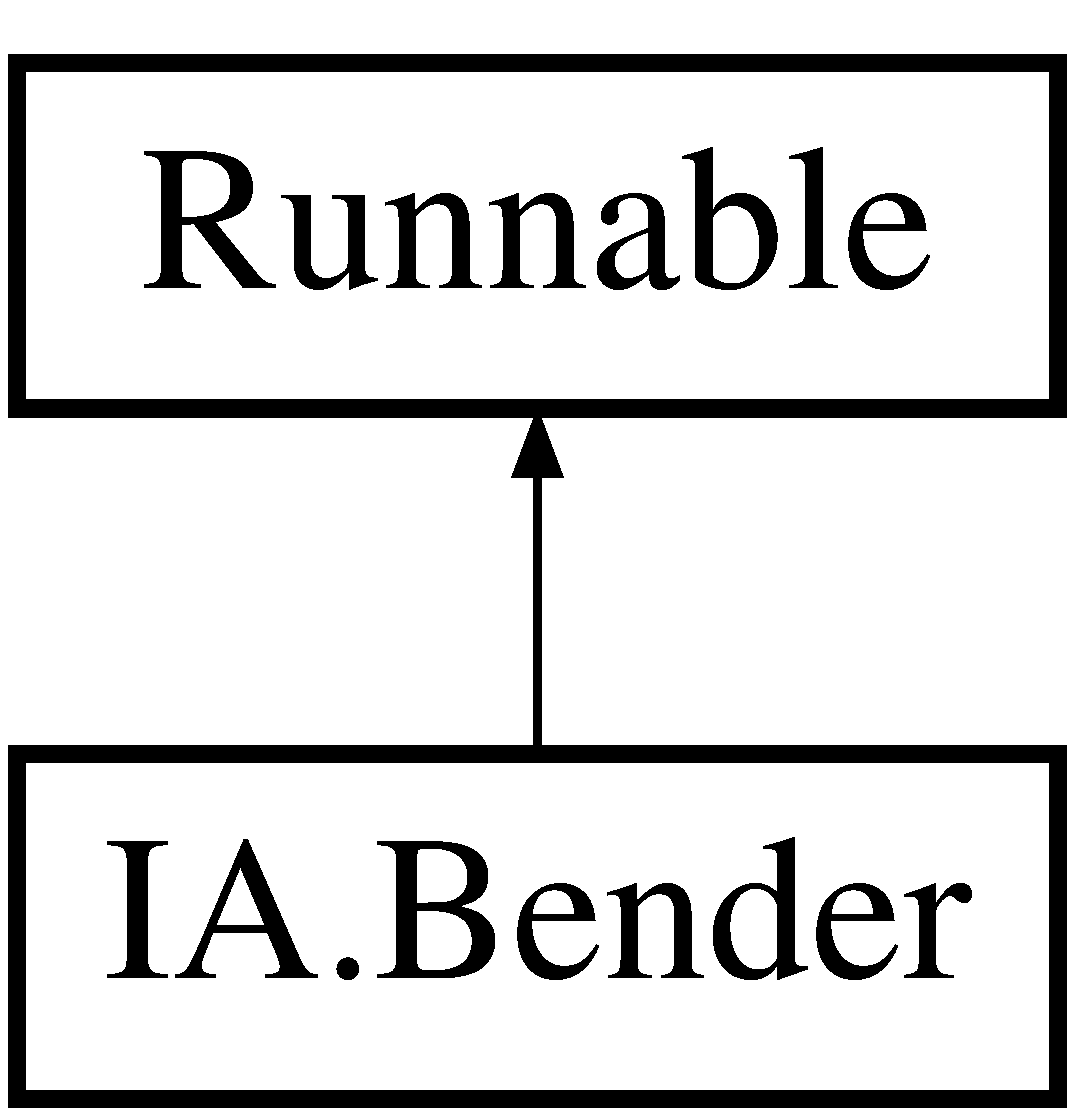
\includegraphics[height=2.000000cm]{class_i_a_1_1_bender}
\end{center}
\end{figure}
\subsection*{Public Member Functions}
\begin{DoxyCompactItemize}
\item 
\hyperlink{class_i_a_1_1_bender_ab961bfaa97015eed15f408a22f442766}{Bender} (\hyperlink{classmain_1_1_main}{Main} master, int cell\+Total)
\item 
void \hyperlink{class_i_a_1_1_bender_a39093dae1a9f2b190e32fc5305a46533}{run} ()
\end{DoxyCompactItemize}


\subsection{Detailed Description}
Classe principale du robot. Possède un état mental B\+DI \begin{DoxyAuthor}{Author}
quentin 
\end{DoxyAuthor}


\subsection{Constructor \& Destructor Documentation}
\hypertarget{class_i_a_1_1_bender_ab961bfaa97015eed15f408a22f442766}{}\label{class_i_a_1_1_bender_ab961bfaa97015eed15f408a22f442766} 
\index{I\+A\+::\+Bender@{I\+A\+::\+Bender}!Bender@{Bender}}
\index{Bender@{Bender}!I\+A\+::\+Bender@{I\+A\+::\+Bender}}
\subsubsection{\texorpdfstring{Bender()}{Bender()}}
{\footnotesize\ttfamily I\+A.\+Bender.\+Bender (\begin{DoxyParamCaption}\item[{\hyperlink{classmain_1_1_main}{Main}}]{master,  }\item[{int}]{cell\+Total }\end{DoxyParamCaption})}

Le constructeur de l\textquotesingle{}objet Aspirateur. En plus d\textquotesingle{}initialiser les attributs \char`\"{}master\char`\"{}, \char`\"{}is\+Explo\+Done\char`\"{} et \char`\"{}cell\+Total\char`\"{}, crée la cellule de départ et l\textquotesingle{}ajoute à la grille.


\begin{DoxyParams}{Parameters}
{\em master} & Référence vers le maître qui instancie tous les threads. Nécessaire afin de mettre à jour l\textquotesingle{}environnement en fonction des actions du robot. \\
\hline
{\em cell\+Total} & Nombre de cellules total dans la grille. Permet au robot de savoir quand terminer la phase d\textquotesingle{}exploration. \\
\hline
\end{DoxyParams}


\subsection{Member Function Documentation}
\hypertarget{class_i_a_1_1_bender_a39093dae1a9f2b190e32fc5305a46533}{}\label{class_i_a_1_1_bender_a39093dae1a9f2b190e32fc5305a46533} 
\index{I\+A\+::\+Bender@{I\+A\+::\+Bender}!run@{run}}
\index{run@{run}!I\+A\+::\+Bender@{I\+A\+::\+Bender}}
\subsubsection{\texorpdfstring{run()}{run()}}
{\footnotesize\ttfamily void I\+A.\+Bender.\+run (\begin{DoxyParamCaption}{ }\end{DoxyParamCaption})}

La méthode \hyperlink{class_i_a_1_1_bender_a39093dae1a9f2b190e32fc5305a46533}{run()} du thread Aspirateur. La routine du robot met à jour ses Beliefs, puis appelle la fonction get\+Desire() afin d\textquotesingle{}obtenir la prochaine tâche à effectuer, puis effectuer cette tâche. 

The documentation for this class was generated from the following file\+:\begin{DoxyCompactItemize}
\item 
I\+A/Bender.\+java\end{DoxyCompactItemize}

\hypertarget{classenvironnement_1_1_cell}{}\section{environnement.\+Cell Class Reference}
\label{classenvironnement_1_1_cell}\index{environnement.\+Cell@{environnement.\+Cell}}
\subsection*{Public Member Functions}
\begin{DoxyCompactItemize}
\item 
\hyperlink{classenvironnement_1_1_cell_ada829b1f91021c63aa07bea9f9f4285c}{Cell} (int r, int c)
\item 
\hyperlink{classenvironnement_1_1_cell_a811f3e78d96ea09509dd67cfd23cde66}{Cell} (int r, int c, Boolean e)
\item 
Boolean \hyperlink{classenvironnement_1_1_cell_a25650d3cbb77512f24039d6ac9d454ba}{get\+Enable} ()
\item 
void \hyperlink{classenvironnement_1_1_cell_a6581171e649b2eca5bf1ebfcdc106ed9}{set\+Enable} (Boolean enable)
\item 
int \hyperlink{classenvironnement_1_1_cell_ab4854841abcb284f9478c921dd3c86d3}{get\+Col} ()
\item 
void \hyperlink{classenvironnement_1_1_cell_a864f6711fd70a6fa132f8c2280db72af}{set\+Col} (int col)
\item 
int \hyperlink{classenvironnement_1_1_cell_a614f23d343407efa4f07156f414522db}{get\+Row} ()
\item 
void \hyperlink{classenvironnement_1_1_cell_a66a02095836f9791548e7ef0547569b5}{set\+Row} (int row)
\item 
Array\+List$<$ \hyperlink{classenvironnement_1_1_object}{Object} $>$ \hyperlink{classenvironnement_1_1_cell_a2423a51a5e48790cea89061c3793357a}{get\+Objects} ()
\item 
void \hyperlink{classenvironnement_1_1_cell_a7a5be16d3f2bd085a86e67d2266680eb}{set\+Objects} (Array\+List$<$ \hyperlink{classenvironnement_1_1_object}{Object} $>$ objects)
\item 
void \hyperlink{classenvironnement_1_1_cell_aedfad655287c0ae1fda977ec15efb6a0}{add\+Object} (\hyperlink{enumenvironnement_1_1_type}{Type} t)
\item 
Boolean \hyperlink{classenvironnement_1_1_cell_ad83c17c96dae12f864af43ad546f86f3}{remove\+Object} (\hyperlink{enumenvironnement_1_1_type}{Type} t)
\item 
void \hyperlink{classenvironnement_1_1_cell_a1844f98b1999045deb72d45c7ec0ff21}{remove\+All\+Objects} ()
\item 
Boolean \hyperlink{classenvironnement_1_1_cell_a3551332fb08fc588ca65714cc7642046}{has\+Object} (\hyperlink{enumenvironnement_1_1_type}{Type} t)
\item 
String \hyperlink{classenvironnement_1_1_cell_ab3f7830b0b36a34150a732d2f17ba66d}{to\+String} ()
\end{DoxyCompactItemize}


\subsection{Detailed Description}
Classe représentant une cellule de la \hyperlink{classenvironnement_1_1_grid}{environnement.\+Grid} \begin{DoxyAuthor}{Author}
Thomas 
\end{DoxyAuthor}


\subsection{Constructor \& Destructor Documentation}
\hypertarget{classenvironnement_1_1_cell_ada829b1f91021c63aa07bea9f9f4285c}{}\label{classenvironnement_1_1_cell_ada829b1f91021c63aa07bea9f9f4285c} 
\index{environnement\+::\+Cell@{environnement\+::\+Cell}!Cell@{Cell}}
\index{Cell@{Cell}!environnement\+::\+Cell@{environnement\+::\+Cell}}
\subsubsection{\texorpdfstring{Cell()}{Cell()}\hspace{0.1cm}{\footnotesize\ttfamily [1/2]}}
{\footnotesize\ttfamily environnement.\+Cell.\+Cell (\begin{DoxyParamCaption}\item[{int}]{r,  }\item[{int}]{c }\end{DoxyParamCaption})}

Constructeur de la classe prenant en paramètre la ligne et la colonne de la cellule 
\begin{DoxyParams}{Parameters}
{\em r} & Ligne de la cellule \\
\hline
{\em c} & Colonne de la cellule \\
\hline
\end{DoxyParams}
\hypertarget{classenvironnement_1_1_cell_a811f3e78d96ea09509dd67cfd23cde66}{}\label{classenvironnement_1_1_cell_a811f3e78d96ea09509dd67cfd23cde66} 
\index{environnement\+::\+Cell@{environnement\+::\+Cell}!Cell@{Cell}}
\index{Cell@{Cell}!environnement\+::\+Cell@{environnement\+::\+Cell}}
\subsubsection{\texorpdfstring{Cell()}{Cell()}\hspace{0.1cm}{\footnotesize\ttfamily [2/2]}}
{\footnotesize\ttfamily environnement.\+Cell.\+Cell (\begin{DoxyParamCaption}\item[{int}]{r,  }\item[{int}]{c,  }\item[{Boolean}]{e }\end{DoxyParamCaption})}

Surcharge du constructeur prenant en compte si la cellule est valable 
\begin{DoxyParams}{Parameters}
{\em r} & Ligne de la cellule \\
\hline
{\em c} & Colonne de la cellule \\
\hline
{\em e} & Si la cellule est valable \\
\hline
\end{DoxyParams}


\subsection{Member Function Documentation}
\hypertarget{classenvironnement_1_1_cell_aedfad655287c0ae1fda977ec15efb6a0}{}\label{classenvironnement_1_1_cell_aedfad655287c0ae1fda977ec15efb6a0} 
\index{environnement\+::\+Cell@{environnement\+::\+Cell}!add\+Object@{add\+Object}}
\index{add\+Object@{add\+Object}!environnement\+::\+Cell@{environnement\+::\+Cell}}
\subsubsection{\texorpdfstring{add\+Object()}{addObject()}}
{\footnotesize\ttfamily void environnement.\+Cell.\+add\+Object (\begin{DoxyParamCaption}\item[{\hyperlink{enumenvironnement_1_1_type}{Type}}]{t }\end{DoxyParamCaption})}

Méthode permettant de rajouter un objet d\textquotesingle{}un certain \hyperlink{}{Type} à la cellule 
\begin{DoxyParams}{Parameters}
{\em t} & Le type de l\textquotesingle{}objet à ajouter \\
\hline
\end{DoxyParams}
\hypertarget{classenvironnement_1_1_cell_ab4854841abcb284f9478c921dd3c86d3}{}\label{classenvironnement_1_1_cell_ab4854841abcb284f9478c921dd3c86d3} 
\index{environnement\+::\+Cell@{environnement\+::\+Cell}!get\+Col@{get\+Col}}
\index{get\+Col@{get\+Col}!environnement\+::\+Cell@{environnement\+::\+Cell}}
\subsubsection{\texorpdfstring{get\+Col()}{getCol()}}
{\footnotesize\ttfamily int environnement.\+Cell.\+get\+Col (\begin{DoxyParamCaption}{ }\end{DoxyParamCaption})}

Getter de la colonne de la cellule \begin{DoxyReturn}{Returns}
La colonne de la cellule 
\end{DoxyReturn}
\hypertarget{classenvironnement_1_1_cell_a25650d3cbb77512f24039d6ac9d454ba}{}\label{classenvironnement_1_1_cell_a25650d3cbb77512f24039d6ac9d454ba} 
\index{environnement\+::\+Cell@{environnement\+::\+Cell}!get\+Enable@{get\+Enable}}
\index{get\+Enable@{get\+Enable}!environnement\+::\+Cell@{environnement\+::\+Cell}}
\subsubsection{\texorpdfstring{get\+Enable()}{getEnable()}}
{\footnotesize\ttfamily Boolean environnement.\+Cell.\+get\+Enable (\begin{DoxyParamCaption}{ }\end{DoxyParamCaption})}

Getter de la validité de la cellule \begin{DoxyReturn}{Returns}
Si la cellule est valable 
\end{DoxyReturn}
\hypertarget{classenvironnement_1_1_cell_a2423a51a5e48790cea89061c3793357a}{}\label{classenvironnement_1_1_cell_a2423a51a5e48790cea89061c3793357a} 
\index{environnement\+::\+Cell@{environnement\+::\+Cell}!get\+Objects@{get\+Objects}}
\index{get\+Objects@{get\+Objects}!environnement\+::\+Cell@{environnement\+::\+Cell}}
\subsubsection{\texorpdfstring{get\+Objects()}{getObjects()}}
{\footnotesize\ttfamily Array\+List$<$\hyperlink{classenvironnement_1_1_object}{Object}$>$ environnement.\+Cell.\+get\+Objects (\begin{DoxyParamCaption}{ }\end{DoxyParamCaption})}

Getter de la liste des objets présents dans la cellule \begin{DoxyReturn}{Returns}
La liste des objets présents dans la cellule 
\end{DoxyReturn}
\hypertarget{classenvironnement_1_1_cell_a614f23d343407efa4f07156f414522db}{}\label{classenvironnement_1_1_cell_a614f23d343407efa4f07156f414522db} 
\index{environnement\+::\+Cell@{environnement\+::\+Cell}!get\+Row@{get\+Row}}
\index{get\+Row@{get\+Row}!environnement\+::\+Cell@{environnement\+::\+Cell}}
\subsubsection{\texorpdfstring{get\+Row()}{getRow()}}
{\footnotesize\ttfamily int environnement.\+Cell.\+get\+Row (\begin{DoxyParamCaption}{ }\end{DoxyParamCaption})}

Getter de la ligne de la cellule \begin{DoxyReturn}{Returns}
La ligne de la cellule 
\end{DoxyReturn}
\hypertarget{classenvironnement_1_1_cell_a3551332fb08fc588ca65714cc7642046}{}\label{classenvironnement_1_1_cell_a3551332fb08fc588ca65714cc7642046} 
\index{environnement\+::\+Cell@{environnement\+::\+Cell}!has\+Object@{has\+Object}}
\index{has\+Object@{has\+Object}!environnement\+::\+Cell@{environnement\+::\+Cell}}
\subsubsection{\texorpdfstring{has\+Object()}{hasObject()}}
{\footnotesize\ttfamily Boolean environnement.\+Cell.\+has\+Object (\begin{DoxyParamCaption}\item[{\hyperlink{enumenvironnement_1_1_type}{Type}}]{t }\end{DoxyParamCaption})}

Méthode permettant de tester si la cellule possède un objet du type passé en paramètre 
\begin{DoxyParams}{Parameters}
{\em t} & Le type de l\textquotesingle{}objet à tester \\
\hline
\end{DoxyParams}
\begin{DoxyReturn}{Returns}
Si le type d\textquotesingle{}objet est présent dans la cellule 
\end{DoxyReturn}
\hypertarget{classenvironnement_1_1_cell_a1844f98b1999045deb72d45c7ec0ff21}{}\label{classenvironnement_1_1_cell_a1844f98b1999045deb72d45c7ec0ff21} 
\index{environnement\+::\+Cell@{environnement\+::\+Cell}!remove\+All\+Objects@{remove\+All\+Objects}}
\index{remove\+All\+Objects@{remove\+All\+Objects}!environnement\+::\+Cell@{environnement\+::\+Cell}}
\subsubsection{\texorpdfstring{remove\+All\+Objects()}{removeAllObjects()}}
{\footnotesize\ttfamily void environnement.\+Cell.\+remove\+All\+Objects (\begin{DoxyParamCaption}{ }\end{DoxyParamCaption})}

Méthode permettant de supprimer tous les objets de la cellule \hypertarget{classenvironnement_1_1_cell_ad83c17c96dae12f864af43ad546f86f3}{}\label{classenvironnement_1_1_cell_ad83c17c96dae12f864af43ad546f86f3} 
\index{environnement\+::\+Cell@{environnement\+::\+Cell}!remove\+Object@{remove\+Object}}
\index{remove\+Object@{remove\+Object}!environnement\+::\+Cell@{environnement\+::\+Cell}}
\subsubsection{\texorpdfstring{remove\+Object()}{removeObject()}}
{\footnotesize\ttfamily Boolean environnement.\+Cell.\+remove\+Object (\begin{DoxyParamCaption}\item[{\hyperlink{enumenvironnement_1_1_type}{Type}}]{t }\end{DoxyParamCaption})}

Méthode permettant de supprimer un objet d\textquotesingle{}un certain \hyperlink{}{Type} de la cellule 
\begin{DoxyParams}{Parameters}
{\em t} & Le type de l\textquotesingle{}objet à supprimer \\
\hline
\end{DoxyParams}
\begin{DoxyReturn}{Returns}
L\textquotesingle{}objet supprimé 
\end{DoxyReturn}
\hypertarget{classenvironnement_1_1_cell_a864f6711fd70a6fa132f8c2280db72af}{}\label{classenvironnement_1_1_cell_a864f6711fd70a6fa132f8c2280db72af} 
\index{environnement\+::\+Cell@{environnement\+::\+Cell}!set\+Col@{set\+Col}}
\index{set\+Col@{set\+Col}!environnement\+::\+Cell@{environnement\+::\+Cell}}
\subsubsection{\texorpdfstring{set\+Col()}{setCol()}}
{\footnotesize\ttfamily void environnement.\+Cell.\+set\+Col (\begin{DoxyParamCaption}\item[{int}]{col }\end{DoxyParamCaption})}

Setter de la colonne de la cellule 
\begin{DoxyParams}{Parameters}
{\em col} & Colonne de la cellule \\
\hline
\end{DoxyParams}
\hypertarget{classenvironnement_1_1_cell_a6581171e649b2eca5bf1ebfcdc106ed9}{}\label{classenvironnement_1_1_cell_a6581171e649b2eca5bf1ebfcdc106ed9} 
\index{environnement\+::\+Cell@{environnement\+::\+Cell}!set\+Enable@{set\+Enable}}
\index{set\+Enable@{set\+Enable}!environnement\+::\+Cell@{environnement\+::\+Cell}}
\subsubsection{\texorpdfstring{set\+Enable()}{setEnable()}}
{\footnotesize\ttfamily void environnement.\+Cell.\+set\+Enable (\begin{DoxyParamCaption}\item[{Boolean}]{enable }\end{DoxyParamCaption})}

Setter de la validité de la cellule 
\begin{DoxyParams}{Parameters}
{\em enable} & Si la cellule est valable \\
\hline
\end{DoxyParams}
\hypertarget{classenvironnement_1_1_cell_a7a5be16d3f2bd085a86e67d2266680eb}{}\label{classenvironnement_1_1_cell_a7a5be16d3f2bd085a86e67d2266680eb} 
\index{environnement\+::\+Cell@{environnement\+::\+Cell}!set\+Objects@{set\+Objects}}
\index{set\+Objects@{set\+Objects}!environnement\+::\+Cell@{environnement\+::\+Cell}}
\subsubsection{\texorpdfstring{set\+Objects()}{setObjects()}}
{\footnotesize\ttfamily void environnement.\+Cell.\+set\+Objects (\begin{DoxyParamCaption}\item[{Array\+List$<$ \hyperlink{classenvironnement_1_1_object}{Object} $>$}]{objects }\end{DoxyParamCaption})}

Setter de la liste des objets présents dans la cellule 
\begin{DoxyParams}{Parameters}
{\em objects} & La liste des objets présents dans la cellule \\
\hline
\end{DoxyParams}
\hypertarget{classenvironnement_1_1_cell_a66a02095836f9791548e7ef0547569b5}{}\label{classenvironnement_1_1_cell_a66a02095836f9791548e7ef0547569b5} 
\index{environnement\+::\+Cell@{environnement\+::\+Cell}!set\+Row@{set\+Row}}
\index{set\+Row@{set\+Row}!environnement\+::\+Cell@{environnement\+::\+Cell}}
\subsubsection{\texorpdfstring{set\+Row()}{setRow()}}
{\footnotesize\ttfamily void environnement.\+Cell.\+set\+Row (\begin{DoxyParamCaption}\item[{int}]{row }\end{DoxyParamCaption})}

Setter de la ligne de la cellule 
\begin{DoxyParams}{Parameters}
{\em row} & La ligne de la cellule \\
\hline
\end{DoxyParams}
\hypertarget{classenvironnement_1_1_cell_ab3f7830b0b36a34150a732d2f17ba66d}{}\label{classenvironnement_1_1_cell_ab3f7830b0b36a34150a732d2f17ba66d} 
\index{environnement\+::\+Cell@{environnement\+::\+Cell}!to\+String@{to\+String}}
\index{to\+String@{to\+String}!environnement\+::\+Cell@{environnement\+::\+Cell}}
\subsubsection{\texorpdfstring{to\+String()}{toString()}}
{\footnotesize\ttfamily String environnement.\+Cell.\+to\+String (\begin{DoxyParamCaption}{ }\end{DoxyParamCaption})}

Méthode utilisée pour identifier la cellule sous forme de chaine de caractères \begin{DoxyReturn}{Returns}
La chaine de caractère identifiant la cellule sour la forme \mbox{[}ligne, colonne\mbox{]} 
\end{DoxyReturn}


The documentation for this class was generated from the following file\+:\begin{DoxyCompactItemize}
\item 
environnement/Cell.\+java\end{DoxyCompactItemize}

\hypertarget{classgraphic_1_1_cell_pane}{}\section{graphic.\+Cell\+Pane Class Reference}
\label{classgraphic_1_1_cell_pane}\index{graphic.\+Cell\+Pane@{graphic.\+Cell\+Pane}}
Inheritance diagram for graphic.\+Cell\+Pane\+:\begin{figure}[H]
\begin{center}
\leavevmode
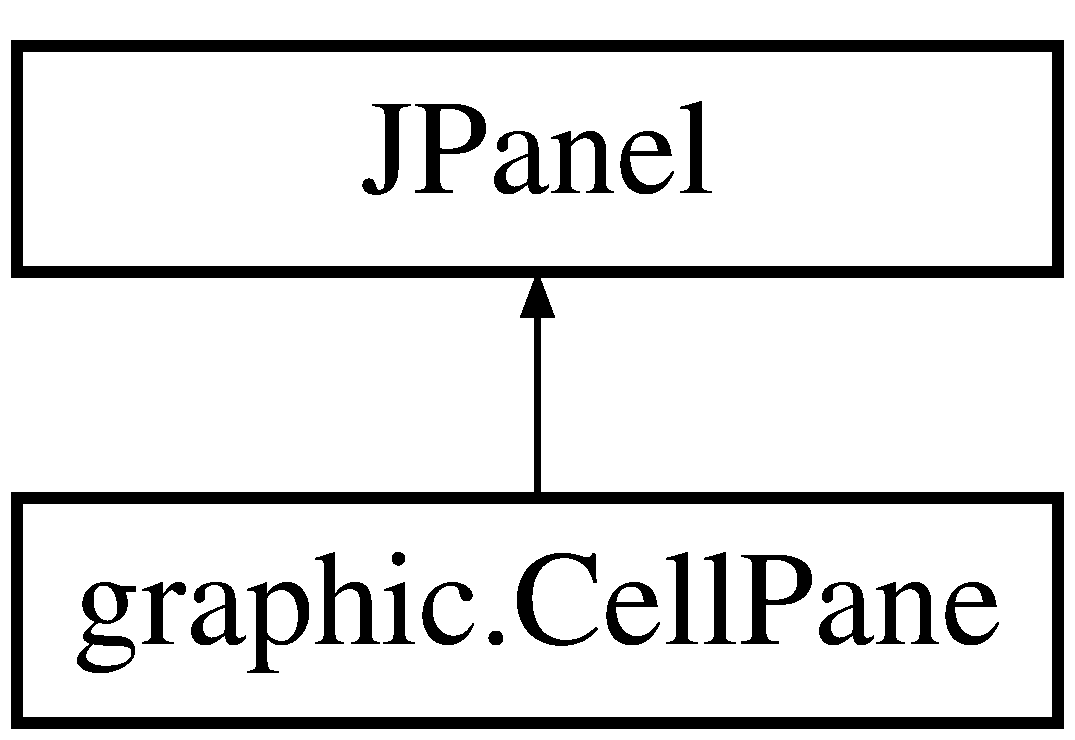
\includegraphics[height=2.000000cm]{classgraphic_1_1_cell_pane}
\end{center}
\end{figure}
\subsection*{Public Member Functions}
\begin{DoxyCompactItemize}
\item 
\hyperlink{classgraphic_1_1_cell_pane_acfa4533330876d91705e1871c854c1f2}{Cell\+Pane} (\hyperlink{classgraphic_1_1_grid_panel}{Grid\+Panel} gp, int x, int y)
\item 
Dimension \hyperlink{classgraphic_1_1_cell_pane_a0fd531a6556674de04015e906aabe03a}{get\+Preferred\+Size} ()
\item 
\hyperlink{classgraphic_1_1_grid_panel}{Grid\+Panel} \hyperlink{classgraphic_1_1_cell_pane_a34a6be4ba7f268bc1cf97abb8133ea21}{get\+Gp} ()
\item 
void \hyperlink{classgraphic_1_1_cell_pane_aa61724c598a72a3b1968bc07bb2c29aa}{set\+Gp} (\hyperlink{classgraphic_1_1_grid_panel}{Grid\+Panel} gp)
\item 
int \hyperlink{classgraphic_1_1_cell_pane_a26561bfa4a8802268c9b081e5c5682f8}{get\+CoordX} ()
\item 
void \hyperlink{classgraphic_1_1_cell_pane_ad2287605b18570f3af59ada0e1feaade}{set\+CoordX} (int coordX)
\item 
int \hyperlink{classgraphic_1_1_cell_pane_a085ea8c70a07a051e103af3c89e66eb2}{get\+CoordY} ()
\item 
void \hyperlink{classgraphic_1_1_cell_pane_a5f6ca9deb28ada5b1442f6b9ecb3b616}{set\+CoordY} (int coordY)
\end{DoxyCompactItemize}


\subsection{Detailed Description}
Classe représant une cellule de la grille \begin{DoxyAuthor}{Author}
Maxime 
\end{DoxyAuthor}


\subsection{Constructor \& Destructor Documentation}
\hypertarget{classgraphic_1_1_cell_pane_acfa4533330876d91705e1871c854c1f2}{}\label{classgraphic_1_1_cell_pane_acfa4533330876d91705e1871c854c1f2} 
\index{graphic\+::\+Cell\+Pane@{graphic\+::\+Cell\+Pane}!Cell\+Pane@{Cell\+Pane}}
\index{Cell\+Pane@{Cell\+Pane}!graphic\+::\+Cell\+Pane@{graphic\+::\+Cell\+Pane}}
\subsubsection{\texorpdfstring{Cell\+Pane()}{CellPane()}}
{\footnotesize\ttfamily graphic.\+Cell\+Pane.\+Cell\+Pane (\begin{DoxyParamCaption}\item[{\hyperlink{classgraphic_1_1_grid_panel}{Grid\+Panel}}]{gp,  }\item[{int}]{x,  }\item[{int}]{y }\end{DoxyParamCaption})}

constructeur de la classe prenant en paramètre sa grille mère, et ses coordonnées x et y 
\begin{DoxyParams}{Parameters}
{\em gp} & = grille mère \\
\hline
{\em x} & = colonne de la cellule \\
\hline
{\em y} & = ligne de la cellule \\
\hline
\end{DoxyParams}
Méthode qui permet de modifier le background lorsque la souris de l\textquotesingle{}utilisateur entre dans la cellule

on remet le fond de la cellule par défaut lorsque l\textquotesingle{}utilisateur sort de la cellule 
\begin{DoxyParams}{Parameters}
{\em e} & \\
\hline
\end{DoxyParams}
on affiche un menu contextuel lorsque l\textquotesingle{}utilisateur clique droit sur la cellule 
\begin{DoxyParams}{Parameters}
{\em e} & \\
\hline
\end{DoxyParams}


\subsection{Member Function Documentation}
\hypertarget{classgraphic_1_1_cell_pane_a26561bfa4a8802268c9b081e5c5682f8}{}\label{classgraphic_1_1_cell_pane_a26561bfa4a8802268c9b081e5c5682f8} 
\index{graphic\+::\+Cell\+Pane@{graphic\+::\+Cell\+Pane}!get\+CoordX@{get\+CoordX}}
\index{get\+CoordX@{get\+CoordX}!graphic\+::\+Cell\+Pane@{graphic\+::\+Cell\+Pane}}
\subsubsection{\texorpdfstring{get\+Coord\+X()}{getCoordX()}}
{\footnotesize\ttfamily int graphic.\+Cell\+Pane.\+get\+CoordX (\begin{DoxyParamCaption}{ }\end{DoxyParamCaption})}

Getter qui retourne la coordonnée X de la cellule \begin{DoxyReturn}{Returns}
the coordX (la colonne) 
\end{DoxyReturn}
\hypertarget{classgraphic_1_1_cell_pane_a085ea8c70a07a051e103af3c89e66eb2}{}\label{classgraphic_1_1_cell_pane_a085ea8c70a07a051e103af3c89e66eb2} 
\index{graphic\+::\+Cell\+Pane@{graphic\+::\+Cell\+Pane}!get\+CoordY@{get\+CoordY}}
\index{get\+CoordY@{get\+CoordY}!graphic\+::\+Cell\+Pane@{graphic\+::\+Cell\+Pane}}
\subsubsection{\texorpdfstring{get\+Coord\+Y()}{getCoordY()}}
{\footnotesize\ttfamily int graphic.\+Cell\+Pane.\+get\+CoordY (\begin{DoxyParamCaption}{ }\end{DoxyParamCaption})}

Getter qui retourne la coordonnée Y de la cellule \begin{DoxyReturn}{Returns}
the coordY (la ligne) 
\end{DoxyReturn}
\hypertarget{classgraphic_1_1_cell_pane_a34a6be4ba7f268bc1cf97abb8133ea21}{}\label{classgraphic_1_1_cell_pane_a34a6be4ba7f268bc1cf97abb8133ea21} 
\index{graphic\+::\+Cell\+Pane@{graphic\+::\+Cell\+Pane}!get\+Gp@{get\+Gp}}
\index{get\+Gp@{get\+Gp}!graphic\+::\+Cell\+Pane@{graphic\+::\+Cell\+Pane}}
\subsubsection{\texorpdfstring{get\+Gp()}{getGp()}}
{\footnotesize\ttfamily \hyperlink{classgraphic_1_1_grid_panel}{Grid\+Panel} graphic.\+Cell\+Pane.\+get\+Gp (\begin{DoxyParamCaption}{ }\end{DoxyParamCaption})}

Getter de la grille mère \begin{DoxyReturn}{Returns}
the gp 
\end{DoxyReturn}
\hypertarget{classgraphic_1_1_cell_pane_a0fd531a6556674de04015e906aabe03a}{}\label{classgraphic_1_1_cell_pane_a0fd531a6556674de04015e906aabe03a} 
\index{graphic\+::\+Cell\+Pane@{graphic\+::\+Cell\+Pane}!get\+Preferred\+Size@{get\+Preferred\+Size}}
\index{get\+Preferred\+Size@{get\+Preferred\+Size}!graphic\+::\+Cell\+Pane@{graphic\+::\+Cell\+Pane}}
\subsubsection{\texorpdfstring{get\+Preferred\+Size()}{getPreferredSize()}}
{\footnotesize\ttfamily Dimension graphic.\+Cell\+Pane.\+get\+Preferred\+Size (\begin{DoxyParamCaption}{ }\end{DoxyParamCaption})}

taille de la cellule \begin{DoxyReturn}{Returns}
la dimension 
\end{DoxyReturn}
\hypertarget{classgraphic_1_1_cell_pane_ad2287605b18570f3af59ada0e1feaade}{}\label{classgraphic_1_1_cell_pane_ad2287605b18570f3af59ada0e1feaade} 
\index{graphic\+::\+Cell\+Pane@{graphic\+::\+Cell\+Pane}!set\+CoordX@{set\+CoordX}}
\index{set\+CoordX@{set\+CoordX}!graphic\+::\+Cell\+Pane@{graphic\+::\+Cell\+Pane}}
\subsubsection{\texorpdfstring{set\+Coord\+X()}{setCoordX()}}
{\footnotesize\ttfamily void graphic.\+Cell\+Pane.\+set\+CoordX (\begin{DoxyParamCaption}\item[{int}]{coordX }\end{DoxyParamCaption})}

Setter qui modifie la coordonnée X de la cellule 
\begin{DoxyParams}{Parameters}
{\em coordX} & the coordX to set (la colonne) \\
\hline
\end{DoxyParams}
\hypertarget{classgraphic_1_1_cell_pane_a5f6ca9deb28ada5b1442f6b9ecb3b616}{}\label{classgraphic_1_1_cell_pane_a5f6ca9deb28ada5b1442f6b9ecb3b616} 
\index{graphic\+::\+Cell\+Pane@{graphic\+::\+Cell\+Pane}!set\+CoordY@{set\+CoordY}}
\index{set\+CoordY@{set\+CoordY}!graphic\+::\+Cell\+Pane@{graphic\+::\+Cell\+Pane}}
\subsubsection{\texorpdfstring{set\+Coord\+Y()}{setCoordY()}}
{\footnotesize\ttfamily void graphic.\+Cell\+Pane.\+set\+CoordY (\begin{DoxyParamCaption}\item[{int}]{coordY }\end{DoxyParamCaption})}

Setter qui permet de modifier la coordonnée Y de la cellule 
\begin{DoxyParams}{Parameters}
{\em coordY} & the coordY to set (la ligne) \\
\hline
\end{DoxyParams}
\hypertarget{classgraphic_1_1_cell_pane_aa61724c598a72a3b1968bc07bb2c29aa}{}\label{classgraphic_1_1_cell_pane_aa61724c598a72a3b1968bc07bb2c29aa} 
\index{graphic\+::\+Cell\+Pane@{graphic\+::\+Cell\+Pane}!set\+Gp@{set\+Gp}}
\index{set\+Gp@{set\+Gp}!graphic\+::\+Cell\+Pane@{graphic\+::\+Cell\+Pane}}
\subsubsection{\texorpdfstring{set\+Gp()}{setGp()}}
{\footnotesize\ttfamily void graphic.\+Cell\+Pane.\+set\+Gp (\begin{DoxyParamCaption}\item[{\hyperlink{classgraphic_1_1_grid_panel}{Grid\+Panel}}]{gp }\end{DoxyParamCaption})}

Setter de la grille mère 
\begin{DoxyParams}{Parameters}
{\em gp} & the gp to set \\
\hline
\end{DoxyParams}


The documentation for this class was generated from the following file\+:\begin{DoxyCompactItemize}
\item 
graphic/Cell\+Pane.\+java\end{DoxyCompactItemize}

\hypertarget{enum_i_a_1_1_desire}{}\section{I\+A.\+Desire Enum Reference}
\label{enum_i_a_1_1_desire}\index{I\+A.\+Desire@{I\+A.\+Desire}}
\subsection*{Public Attributes}
\begin{DoxyCompactItemize}
\item 
\hypertarget{enum_i_a_1_1_desire_a76a68fbecf4b23f292c4beed7758373d}{}\label{enum_i_a_1_1_desire_a76a68fbecf4b23f292c4beed7758373d} 
{\bfseries P\+I\+CK}
\item 
\hypertarget{enum_i_a_1_1_desire_ae441608f9f2d8d07b1dfc452d1202c97}{}\label{enum_i_a_1_1_desire_ae441608f9f2d8d07b1dfc452d1202c97} 
{\bfseries C\+L\+E\+AN}
\item 
\hypertarget{enum_i_a_1_1_desire_a37a88a72c533c4e88cbbabd81105e335}{}\label{enum_i_a_1_1_desire_a37a88a72c533c4e88cbbabd81105e335} 
{\bfseries G\+E\+T\+N\+E\+W\+G\+O\+AL}
\item 
\hypertarget{enum_i_a_1_1_desire_a07c89126c6039806c8d192136733d7e9}{}\label{enum_i_a_1_1_desire_a07c89126c6039806c8d192136733d7e9} 
{\bfseries E\+X\+P\+L\+O\+RE}
\end{DoxyCompactItemize}


\subsection{Detailed Description}
\begin{DoxyAuthor}{Author}
quentin 
\end{DoxyAuthor}


The documentation for this enum was generated from the following file\+:\begin{DoxyCompactItemize}
\item 
I\+A/Desire.\+java\end{DoxyCompactItemize}

\hypertarget{enum_i_a_1_1_direction}{}\section{I\+A.\+Direction Enum Reference}
\label{enum_i_a_1_1_direction}\index{I\+A.\+Direction@{I\+A.\+Direction}}
\subsection*{Public Attributes}
\begin{DoxyCompactItemize}
\item 
\hypertarget{enum_i_a_1_1_direction_a4b8fa637cb73943c3622ff1e533e20bd}{}\label{enum_i_a_1_1_direction_a4b8fa637cb73943c3622ff1e533e20bd} 
{\bfseries L\+E\+FT}
\item 
\hypertarget{enum_i_a_1_1_direction_a708c98aed0edef7cfe31b4aff0d527fe}{}\label{enum_i_a_1_1_direction_a708c98aed0edef7cfe31b4aff0d527fe} 
{\bfseries R\+I\+G\+HT}
\item 
\hypertarget{enum_i_a_1_1_direction_a2dfd287aba6abd714fd190e0517ff85e}{}\label{enum_i_a_1_1_direction_a2dfd287aba6abd714fd190e0517ff85e} 
{\bfseries UP}
\end{DoxyCompactItemize}


\subsection{Detailed Description}
\begin{DoxyAuthor}{Author}
quentin 
\end{DoxyAuthor}


The documentation for this enum was generated from the following file\+:\begin{DoxyCompactItemize}
\item 
I\+A/Direction.\+java\end{DoxyCompactItemize}

\hypertarget{classenvironnement_1_1_environnement}{}\section{environnement.\+Environnement Class Reference}
\label{classenvironnement_1_1_environnement}\index{environnement.\+Environnement@{environnement.\+Environnement}}
Inheritance diagram for environnement.\+Environnement\+:\begin{figure}[H]
\begin{center}
\leavevmode
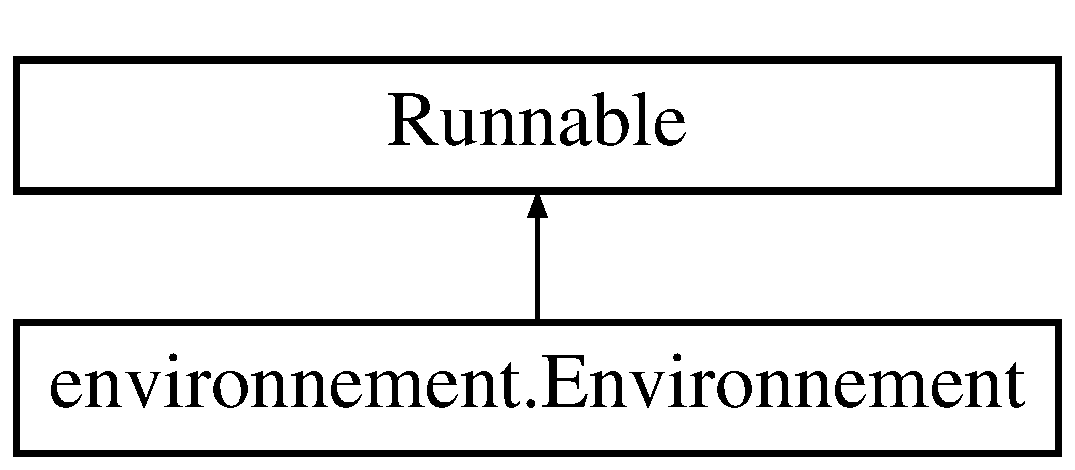
\includegraphics[height=2.000000cm]{classenvironnement_1_1_environnement}
\end{center}
\end{figure}
\subsection*{Public Member Functions}
\begin{DoxyCompactItemize}
\item 
\hyperlink{classenvironnement_1_1_environnement_a664559901643eb5f45ddbf1ec082696b}{Environnement} (\hyperlink{classmain_1_1_main}{Main} main)
\item 
void \hyperlink{classenvironnement_1_1_environnement_a5b7c3fb51c2af94754725667c9a34098}{run} ()
\item 
\hyperlink{classenvironnement_1_1_cell}{Cell} \hyperlink{classenvironnement_1_1_environnement_aa11c05d0dd261136c31224419ecb037a}{get\+Random\+Cell} ()
\item 
int \hyperlink{classenvironnement_1_1_environnement_accb38c1ebc21db442c06f1c39f658853}{get\+Percentage\+Dust} ()
\item 
void \hyperlink{classenvironnement_1_1_environnement_ade3736e361839278d989c81627623b39}{set\+Percentage\+Dust} (int percentage\+Dust)
\item 
int \hyperlink{classenvironnement_1_1_environnement_ab7f263c3832088e66b3e0b2b27882580}{get\+Percentage\+Jewel} ()
\item 
void \hyperlink{classenvironnement_1_1_environnement_a9c0702025cafba8d78596edfb00e1f42}{set\+Percentage\+Jewel} (int percentage\+Jewel)
\item 
int \hyperlink{classenvironnement_1_1_environnement_a93730fe27fd562b41e84c6ae7272c2f1}{get\+Seconds\+To\+Loop} ()
\item 
void \hyperlink{classenvironnement_1_1_environnement_a7d2dde8f8108918651f8f8f8a4bfcdf5}{set\+Seconds\+To\+Loop} (int seconds\+To\+Loop)
\item 
\hyperlink{classenvironnement_1_1_grid}{Grid} \hyperlink{classenvironnement_1_1_environnement_addd77a3e76cf5eb6c3b0270916e4812a}{get\+Grid} ()
\end{DoxyCompactItemize}


\subsection{Detailed Description}
Classe principale de l\textquotesingle{}environnement. Contient les informations générales relatives à l\textquotesingle{}environnement telles que la probabilité d\textquotesingle{}apparition de poussières, le temps entre chaque boucle de tentative d\textquotesingle{}apparition, etc. \begin{DoxyAuthor}{Author}
Thomas 
\end{DoxyAuthor}


\subsection{Constructor \& Destructor Documentation}
\hypertarget{classenvironnement_1_1_environnement_a664559901643eb5f45ddbf1ec082696b}{}\label{classenvironnement_1_1_environnement_a664559901643eb5f45ddbf1ec082696b} 
\index{environnement\+::\+Environnement@{environnement\+::\+Environnement}!Environnement@{Environnement}}
\index{Environnement@{Environnement}!environnement\+::\+Environnement@{environnement\+::\+Environnement}}
\subsubsection{\texorpdfstring{Environnement()}{Environnement()}}
{\footnotesize\ttfamily environnement.\+Environnement.\+Environnement (\begin{DoxyParamCaption}\item[{\hyperlink{classmain_1_1_main}{Main}}]{main }\end{DoxyParamCaption})}

Constructeur de la classe 
\begin{DoxyParams}{Parameters}
{\em main} & Classe principale de l\textquotesingle{}application utilisée comme interface \\
\hline
\end{DoxyParams}


\subsection{Member Function Documentation}
\hypertarget{classenvironnement_1_1_environnement_addd77a3e76cf5eb6c3b0270916e4812a}{}\label{classenvironnement_1_1_environnement_addd77a3e76cf5eb6c3b0270916e4812a} 
\index{environnement\+::\+Environnement@{environnement\+::\+Environnement}!get\+Grid@{get\+Grid}}
\index{get\+Grid@{get\+Grid}!environnement\+::\+Environnement@{environnement\+::\+Environnement}}
\subsubsection{\texorpdfstring{get\+Grid()}{getGrid()}}
{\footnotesize\ttfamily \hyperlink{classenvironnement_1_1_grid}{Grid} environnement.\+Environnement.\+get\+Grid (\begin{DoxyParamCaption}{ }\end{DoxyParamCaption})}

Getter de la \hyperlink{}{grid} de l\textquotesingle{}environnement \begin{DoxyReturn}{Returns}
La \hyperlink{}{grid} de l\textquotesingle{}environnement 
\end{DoxyReturn}
\hypertarget{classenvironnement_1_1_environnement_accb38c1ebc21db442c06f1c39f658853}{}\label{classenvironnement_1_1_environnement_accb38c1ebc21db442c06f1c39f658853} 
\index{environnement\+::\+Environnement@{environnement\+::\+Environnement}!get\+Percentage\+Dust@{get\+Percentage\+Dust}}
\index{get\+Percentage\+Dust@{get\+Percentage\+Dust}!environnement\+::\+Environnement@{environnement\+::\+Environnement}}
\subsubsection{\texorpdfstring{get\+Percentage\+Dust()}{getPercentageDust()}}
{\footnotesize\ttfamily int environnement.\+Environnement.\+get\+Percentage\+Dust (\begin{DoxyParamCaption}{ }\end{DoxyParamCaption})}

Getter de la probabilité d\textquotesingle{}apparition de poussière \begin{DoxyReturn}{Returns}
La probabilité d\textquotesingle{}apparition de poussière 
\end{DoxyReturn}
\hypertarget{classenvironnement_1_1_environnement_ab7f263c3832088e66b3e0b2b27882580}{}\label{classenvironnement_1_1_environnement_ab7f263c3832088e66b3e0b2b27882580} 
\index{environnement\+::\+Environnement@{environnement\+::\+Environnement}!get\+Percentage\+Jewel@{get\+Percentage\+Jewel}}
\index{get\+Percentage\+Jewel@{get\+Percentage\+Jewel}!environnement\+::\+Environnement@{environnement\+::\+Environnement}}
\subsubsection{\texorpdfstring{get\+Percentage\+Jewel()}{getPercentageJewel()}}
{\footnotesize\ttfamily int environnement.\+Environnement.\+get\+Percentage\+Jewel (\begin{DoxyParamCaption}{ }\end{DoxyParamCaption})}

Getter de la probabilité d\textquotesingle{}apparition de bijou \begin{DoxyReturn}{Returns}
La probabilité d\textquotesingle{}apparition de bijou 
\end{DoxyReturn}
\hypertarget{classenvironnement_1_1_environnement_aa11c05d0dd261136c31224419ecb037a}{}\label{classenvironnement_1_1_environnement_aa11c05d0dd261136c31224419ecb037a} 
\index{environnement\+::\+Environnement@{environnement\+::\+Environnement}!get\+Random\+Cell@{get\+Random\+Cell}}
\index{get\+Random\+Cell@{get\+Random\+Cell}!environnement\+::\+Environnement@{environnement\+::\+Environnement}}
\subsubsection{\texorpdfstring{get\+Random\+Cell()}{getRandomCell()}}
{\footnotesize\ttfamily \hyperlink{classenvironnement_1_1_cell}{Cell} environnement.\+Environnement.\+get\+Random\+Cell (\begin{DoxyParamCaption}{ }\end{DoxyParamCaption})}

Méthode permettant de récupérer une cellule aléatoire dans la grille \begin{DoxyReturn}{Returns}
Une cellule de la grille étant enable 
\end{DoxyReturn}
\hypertarget{classenvironnement_1_1_environnement_a93730fe27fd562b41e84c6ae7272c2f1}{}\label{classenvironnement_1_1_environnement_a93730fe27fd562b41e84c6ae7272c2f1} 
\index{environnement\+::\+Environnement@{environnement\+::\+Environnement}!get\+Seconds\+To\+Loop@{get\+Seconds\+To\+Loop}}
\index{get\+Seconds\+To\+Loop@{get\+Seconds\+To\+Loop}!environnement\+::\+Environnement@{environnement\+::\+Environnement}}
\subsubsection{\texorpdfstring{get\+Seconds\+To\+Loop()}{getSecondsToLoop()}}
{\footnotesize\ttfamily int environnement.\+Environnement.\+get\+Seconds\+To\+Loop (\begin{DoxyParamCaption}{ }\end{DoxyParamCaption})}

Getter du temps entre chaque boucle \begin{DoxyReturn}{Returns}
Le temps entre chaque boucle en seconde 
\end{DoxyReturn}
\hypertarget{classenvironnement_1_1_environnement_a5b7c3fb51c2af94754725667c9a34098}{}\label{classenvironnement_1_1_environnement_a5b7c3fb51c2af94754725667c9a34098} 
\index{environnement\+::\+Environnement@{environnement\+::\+Environnement}!run@{run}}
\index{run@{run}!environnement\+::\+Environnement@{environnement\+::\+Environnement}}
\subsubsection{\texorpdfstring{run()}{run()}}
{\footnotesize\ttfamily void environnement.\+Environnement.\+run (\begin{DoxyParamCaption}{ }\end{DoxyParamCaption})}

Méthode principale de la classe. Génère la grille puis tant que \hyperlink{}{run} est vrai génère des poussières et des bijoux. \hypertarget{classenvironnement_1_1_environnement_ade3736e361839278d989c81627623b39}{}\label{classenvironnement_1_1_environnement_ade3736e361839278d989c81627623b39} 
\index{environnement\+::\+Environnement@{environnement\+::\+Environnement}!set\+Percentage\+Dust@{set\+Percentage\+Dust}}
\index{set\+Percentage\+Dust@{set\+Percentage\+Dust}!environnement\+::\+Environnement@{environnement\+::\+Environnement}}
\subsubsection{\texorpdfstring{set\+Percentage\+Dust()}{setPercentageDust()}}
{\footnotesize\ttfamily void environnement.\+Environnement.\+set\+Percentage\+Dust (\begin{DoxyParamCaption}\item[{int}]{percentage\+Dust }\end{DoxyParamCaption})}

Setter de la probabilité d\textquotesingle{}apparition de poussière 
\begin{DoxyParams}{Parameters}
{\em percentage\+Dust} & La probabilité d\textquotesingle{}apparition de poussière \\
\hline
\end{DoxyParams}
\hypertarget{classenvironnement_1_1_environnement_a9c0702025cafba8d78596edfb00e1f42}{}\label{classenvironnement_1_1_environnement_a9c0702025cafba8d78596edfb00e1f42} 
\index{environnement\+::\+Environnement@{environnement\+::\+Environnement}!set\+Percentage\+Jewel@{set\+Percentage\+Jewel}}
\index{set\+Percentage\+Jewel@{set\+Percentage\+Jewel}!environnement\+::\+Environnement@{environnement\+::\+Environnement}}
\subsubsection{\texorpdfstring{set\+Percentage\+Jewel()}{setPercentageJewel()}}
{\footnotesize\ttfamily void environnement.\+Environnement.\+set\+Percentage\+Jewel (\begin{DoxyParamCaption}\item[{int}]{percentage\+Jewel }\end{DoxyParamCaption})}

Setter de la probabilité d\textquotesingle{}apparition de bijou 
\begin{DoxyParams}{Parameters}
{\em percentage\+Jewel} & La probabilité d\textquotesingle{}apparition de bijou \\
\hline
\end{DoxyParams}
\hypertarget{classenvironnement_1_1_environnement_a7d2dde8f8108918651f8f8f8a4bfcdf5}{}\label{classenvironnement_1_1_environnement_a7d2dde8f8108918651f8f8f8a4bfcdf5} 
\index{environnement\+::\+Environnement@{environnement\+::\+Environnement}!set\+Seconds\+To\+Loop@{set\+Seconds\+To\+Loop}}
\index{set\+Seconds\+To\+Loop@{set\+Seconds\+To\+Loop}!environnement\+::\+Environnement@{environnement\+::\+Environnement}}
\subsubsection{\texorpdfstring{set\+Seconds\+To\+Loop()}{setSecondsToLoop()}}
{\footnotesize\ttfamily void environnement.\+Environnement.\+set\+Seconds\+To\+Loop (\begin{DoxyParamCaption}\item[{int}]{seconds\+To\+Loop }\end{DoxyParamCaption})}

Setter du temps entre chaque boucle 
\begin{DoxyParams}{Parameters}
{\em seconds\+To\+Loop} & Le temps entre chaque boucle en seconde \\
\hline
\end{DoxyParams}


The documentation for this class was generated from the following file\+:\begin{DoxyCompactItemize}
\item 
environnement/Environnement.\+java\end{DoxyCompactItemize}

\hypertarget{classenvironnement_1_1_grid}{}\section{environnement.\+Grid Class Reference}
\label{classenvironnement_1_1_grid}\index{environnement.\+Grid@{environnement.\+Grid}}
\subsection*{Public Member Functions}
\begin{DoxyCompactItemize}
\item 
\hyperlink{classenvironnement_1_1_grid_a1757a9849685f20e0bb3bd84a3cf9cb7}{Grid} ()
\item 
\hyperlink{classenvironnement_1_1_cell}{Cell} \hyperlink{classenvironnement_1_1_grid_a81df13c46a58ff1f2accb6debafcced7}{get\+Cell} (int r, int c)
\item 
Array\+List$<$ \hyperlink{classenvironnement_1_1_cell}{Cell} $>$ \hyperlink{classenvironnement_1_1_grid_abaf214d02e4a27765bb266d5e46741de}{get\+Cells} ()
\item 
void \hyperlink{classenvironnement_1_1_grid_a1ea7cb1aa53fa6c45291ad29349731b2}{set\+Cells} (Array\+List$<$ \hyperlink{classenvironnement_1_1_cell}{Cell} $>$ cells)
\end{DoxyCompactItemize}


\subsection{Detailed Description}
Classe représentant la grille de l\textquotesingle{}environnement \begin{DoxyAuthor}{Author}
Thomas 
\end{DoxyAuthor}


\subsection{Constructor \& Destructor Documentation}
\hypertarget{classenvironnement_1_1_grid_a1757a9849685f20e0bb3bd84a3cf9cb7}{}\label{classenvironnement_1_1_grid_a1757a9849685f20e0bb3bd84a3cf9cb7} 
\index{environnement\+::\+Grid@{environnement\+::\+Grid}!Grid@{Grid}}
\index{Grid@{Grid}!environnement\+::\+Grid@{environnement\+::\+Grid}}
\subsubsection{\texorpdfstring{Grid()}{Grid()}}
{\footnotesize\ttfamily environnement.\+Grid.\+Grid (\begin{DoxyParamCaption}{ }\end{DoxyParamCaption})}

Constructeur de la grille X \+: 0 1 2 3 4 Y \+: 0 $\vert$ $\vert$ $\vert$ $\vert$ 1 $\vert$ $\vert$ $\vert$ $\vert$ $\vert$ $\vert$ 2 $\vert$ $\vert$ $\vert$ $\vert$ Crée toutes les cellules nécessaires et mets les cellules situées en \mbox{[}0;3\mbox{]}, \mbox{[}0;4\mbox{]}, \mbox{[}2;3\mbox{]} et \mbox{[}2;4\mbox{]} en non valable 

\subsection{Member Function Documentation}
\hypertarget{classenvironnement_1_1_grid_a81df13c46a58ff1f2accb6debafcced7}{}\label{classenvironnement_1_1_grid_a81df13c46a58ff1f2accb6debafcced7} 
\index{environnement\+::\+Grid@{environnement\+::\+Grid}!get\+Cell@{get\+Cell}}
\index{get\+Cell@{get\+Cell}!environnement\+::\+Grid@{environnement\+::\+Grid}}
\subsubsection{\texorpdfstring{get\+Cell()}{getCell()}}
{\footnotesize\ttfamily \hyperlink{classenvironnement_1_1_cell}{Cell} environnement.\+Grid.\+get\+Cell (\begin{DoxyParamCaption}\item[{int}]{r,  }\item[{int}]{c }\end{DoxyParamCaption})}

Getter d\textquotesingle{}une cellule précise dans la grille 
\begin{DoxyParams}{Parameters}
{\em r} & Ligne de la cellule souhaitée \\
\hline
{\em c} & Colonne de la cellule souhaitée \\
\hline
\end{DoxyParams}
\begin{DoxyReturn}{Returns}
La cellule souhaitée si existante null sinon 
\end{DoxyReturn}
\hypertarget{classenvironnement_1_1_grid_abaf214d02e4a27765bb266d5e46741de}{}\label{classenvironnement_1_1_grid_abaf214d02e4a27765bb266d5e46741de} 
\index{environnement\+::\+Grid@{environnement\+::\+Grid}!get\+Cells@{get\+Cells}}
\index{get\+Cells@{get\+Cells}!environnement\+::\+Grid@{environnement\+::\+Grid}}
\subsubsection{\texorpdfstring{get\+Cells()}{getCells()}}
{\footnotesize\ttfamily Array\+List$<$\hyperlink{classenvironnement_1_1_cell}{Cell}$>$ environnement.\+Grid.\+get\+Cells (\begin{DoxyParamCaption}{ }\end{DoxyParamCaption})}

Getter de toutes les cellules présentes dans la grille \begin{DoxyReturn}{Returns}
Les cellules de la grille 
\end{DoxyReturn}
\hypertarget{classenvironnement_1_1_grid_a1ea7cb1aa53fa6c45291ad29349731b2}{}\label{classenvironnement_1_1_grid_a1ea7cb1aa53fa6c45291ad29349731b2} 
\index{environnement\+::\+Grid@{environnement\+::\+Grid}!set\+Cells@{set\+Cells}}
\index{set\+Cells@{set\+Cells}!environnement\+::\+Grid@{environnement\+::\+Grid}}
\subsubsection{\texorpdfstring{set\+Cells()}{setCells()}}
{\footnotesize\ttfamily void environnement.\+Grid.\+set\+Cells (\begin{DoxyParamCaption}\item[{Array\+List$<$ \hyperlink{classenvironnement_1_1_cell}{Cell} $>$}]{cells }\end{DoxyParamCaption})}

Setter de toutes les cellules présentes dans la grille 
\begin{DoxyParams}{Parameters}
{\em cells} & Les cellules de la grille \\
\hline
\end{DoxyParams}


The documentation for this class was generated from the following file\+:\begin{DoxyCompactItemize}
\item 
environnement/Grid.\+java\end{DoxyCompactItemize}

\hypertarget{classgraphic_1_1_grid_panel}{}\section{graphic.\+Grid\+Panel Class Reference}
\label{classgraphic_1_1_grid_panel}\index{graphic.\+Grid\+Panel@{graphic.\+Grid\+Panel}}
Inheritance diagram for graphic.\+Grid\+Panel\+:\begin{figure}[H]
\begin{center}
\leavevmode
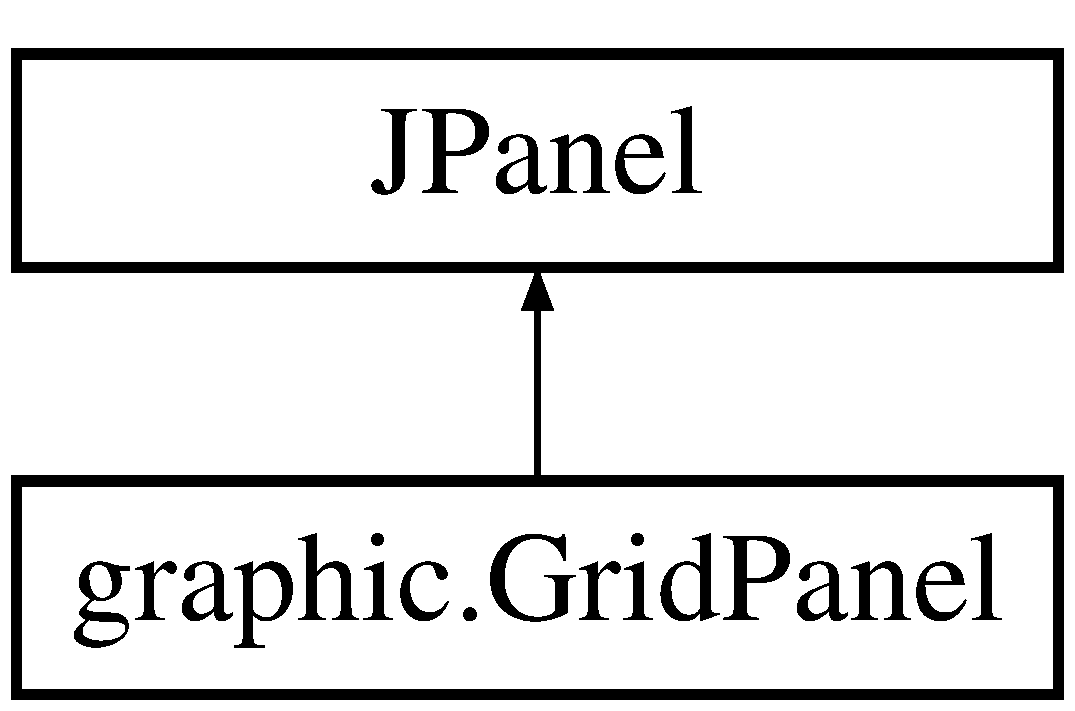
\includegraphics[height=2.000000cm]{classgraphic_1_1_grid_panel}
\end{center}
\end{figure}
\subsection*{Public Member Functions}
\begin{DoxyCompactItemize}
\item 
void \hyperlink{classgraphic_1_1_grid_panel_a3ac9e3dc1d58bee96e2d8c93582542f8}{initialize} (\hyperlink{classgraphic_1_1_main}{graphic.\+Main} main)
\item 
void \hyperlink{classgraphic_1_1_grid_panel_a45010afc7fdcbcd0a4793c9d1e3b9130}{addJ} (int x, int y)
\item 
void \hyperlink{classgraphic_1_1_grid_panel_add084a73d4c1597c56ee83c177c84ea8}{delJ} (int x, int y)
\item 
void \hyperlink{classgraphic_1_1_grid_panel_ac875580b8be1c0b3f2c895352a48a70b}{addD} (int x, int y)
\item 
void \hyperlink{classgraphic_1_1_grid_panel_a8443ee0249f33bbf63bcc45736096a13}{delD} (int x, int y)
\item 
void \hyperlink{classgraphic_1_1_grid_panel_ab1010c154b3bdf06ef05fdd37e18b7bb}{addR} (int x, int y)
\item 
void \hyperlink{classgraphic_1_1_grid_panel_ad114a8a30536087a1dfa6c0df00cdc69}{delR} (int x, int y)
\item 
void \hyperlink{classgraphic_1_1_grid_panel_a0f8dbc4fcd8aa46debd567bccde7abec}{mvtR} (int exX, int exY, int x, int y)
\item 
int \hyperlink{classgraphic_1_1_grid_panel_a76a411ada1cd50f1a9923b55b366c800}{num\+Compo} (int x, int y)
\item 
\hyperlink{classgraphic_1_1_cell_pane}{Cell\+Pane} \hyperlink{classgraphic_1_1_grid_panel_a541bf9099ceafbd082dd5c986af1cadf}{crea\+Cell} (int num\+Cell, int x, int y)
\item 
Border \hyperlink{classgraphic_1_1_grid_panel_ad1d3cae8c7aef1a90c84c74daa07ede3}{f\+Bord} (int num\+Cell)
\item 
\hyperlink{classgraphic_1_1_main}{graphic.\+Main} \hyperlink{classgraphic_1_1_grid_panel_aef759da0374166debd9b42682d17ff5f}{get\+Main} ()
\item 
void \hyperlink{classgraphic_1_1_grid_panel_ac4091164ae46504588cbeb9f22430de0}{set\+Main} (\hyperlink{classgraphic_1_1_main}{graphic.\+Main} main)
\end{DoxyCompactItemize}
\subsection*{Public Attributes}
\begin{DoxyCompactItemize}
\item 
int \mbox{[}$\,$\mbox{]} \hyperlink{classgraphic_1_1_grid_panel_a03acd6ba4608c434fead05a4c37d170a}{etat} = new int\mbox{[}11\mbox{]}
\item 
boolean \hyperlink{classgraphic_1_1_grid_panel_a6c9676cf3ad0b634aea1c48b745d5046}{robot}
\end{DoxyCompactItemize}


\subsection{Detailed Description}
Classe représentant la grille de l\textquotesingle{}interface graphique \begin{DoxyAuthor}{Author}
Maxime 
\end{DoxyAuthor}


\subsection{Member Function Documentation}
\hypertarget{classgraphic_1_1_grid_panel_ac875580b8be1c0b3f2c895352a48a70b}{}\label{classgraphic_1_1_grid_panel_ac875580b8be1c0b3f2c895352a48a70b} 
\index{graphic\+::\+Grid\+Panel@{graphic\+::\+Grid\+Panel}!addD@{addD}}
\index{addD@{addD}!graphic\+::\+Grid\+Panel@{graphic\+::\+Grid\+Panel}}
\subsubsection{\texorpdfstring{add\+D()}{addD()}}
{\footnotesize\ttfamily void graphic.\+Grid\+Panel.\+addD (\begin{DoxyParamCaption}\item[{int}]{x,  }\item[{int}]{y }\end{DoxyParamCaption})}

Méthode qui ajoute de la poussière en position passé en paramètre 
\begin{DoxyParams}{Parameters}
{\em x} & = la colonne \\
\hline
{\em y} & = la ligne \\
\hline
\end{DoxyParams}
\hypertarget{classgraphic_1_1_grid_panel_a45010afc7fdcbcd0a4793c9d1e3b9130}{}\label{classgraphic_1_1_grid_panel_a45010afc7fdcbcd0a4793c9d1e3b9130} 
\index{graphic\+::\+Grid\+Panel@{graphic\+::\+Grid\+Panel}!addJ@{addJ}}
\index{addJ@{addJ}!graphic\+::\+Grid\+Panel@{graphic\+::\+Grid\+Panel}}
\subsubsection{\texorpdfstring{add\+J()}{addJ()}}
{\footnotesize\ttfamily void graphic.\+Grid\+Panel.\+addJ (\begin{DoxyParamCaption}\item[{int}]{x,  }\item[{int}]{y }\end{DoxyParamCaption})}

méthode qui permet d\textquotesingle{}ajouter un bijou en position x et y 
\begin{DoxyParams}{Parameters}
{\em x} & = la colonne où placer le bijou \\
\hline
{\em y} & = la ligne où placer le bijou \\
\hline
\end{DoxyParams}
\hypertarget{classgraphic_1_1_grid_panel_ab1010c154b3bdf06ef05fdd37e18b7bb}{}\label{classgraphic_1_1_grid_panel_ab1010c154b3bdf06ef05fdd37e18b7bb} 
\index{graphic\+::\+Grid\+Panel@{graphic\+::\+Grid\+Panel}!addR@{addR}}
\index{addR@{addR}!graphic\+::\+Grid\+Panel@{graphic\+::\+Grid\+Panel}}
\subsubsection{\texorpdfstring{add\+R()}{addR()}}
{\footnotesize\ttfamily void graphic.\+Grid\+Panel.\+addR (\begin{DoxyParamCaption}\item[{int}]{x,  }\item[{int}]{y }\end{DoxyParamCaption})}

Méthode permettant d\textquotesingle{}ajouter le robot suivant les coordonnées passées en paramètre 
\begin{DoxyParams}{Parameters}
{\em x} & = la colonne \\
\hline
{\em y} & = la ligne \\
\hline
\end{DoxyParams}
\hypertarget{classgraphic_1_1_grid_panel_a541bf9099ceafbd082dd5c986af1cadf}{}\label{classgraphic_1_1_grid_panel_a541bf9099ceafbd082dd5c986af1cadf} 
\index{graphic\+::\+Grid\+Panel@{graphic\+::\+Grid\+Panel}!crea\+Cell@{crea\+Cell}}
\index{crea\+Cell@{crea\+Cell}!graphic\+::\+Grid\+Panel@{graphic\+::\+Grid\+Panel}}
\subsubsection{\texorpdfstring{crea\+Cell()}{creaCell()}}
{\footnotesize\ttfamily \hyperlink{classgraphic_1_1_cell_pane}{Cell\+Pane} graphic.\+Grid\+Panel.\+crea\+Cell (\begin{DoxyParamCaption}\item[{int}]{num\+Cell,  }\item[{int}]{x,  }\item[{int}]{y }\end{DoxyParamCaption})}

Méthode pour créer une cellule 
\begin{DoxyParams}{Parameters}
{\em num\+Cell} & \\
\hline
\end{DoxyParams}
\begin{DoxyReturn}{Returns}
la cellule créée 
\end{DoxyReturn}
\hypertarget{classgraphic_1_1_grid_panel_a8443ee0249f33bbf63bcc45736096a13}{}\label{classgraphic_1_1_grid_panel_a8443ee0249f33bbf63bcc45736096a13} 
\index{graphic\+::\+Grid\+Panel@{graphic\+::\+Grid\+Panel}!delD@{delD}}
\index{delD@{delD}!graphic\+::\+Grid\+Panel@{graphic\+::\+Grid\+Panel}}
\subsubsection{\texorpdfstring{del\+D()}{delD()}}
{\footnotesize\ttfamily void graphic.\+Grid\+Panel.\+delD (\begin{DoxyParamCaption}\item[{int}]{x,  }\item[{int}]{y }\end{DoxyParamCaption})}

Méthode permettant d\textquotesingle{}enlever une poussière suivant les coordonnées passées en paramètre 
\begin{DoxyParams}{Parameters}
{\em x} & = la colonne \\
\hline
{\em y} & = la ligne \\
\hline
\end{DoxyParams}
\hypertarget{classgraphic_1_1_grid_panel_add084a73d4c1597c56ee83c177c84ea8}{}\label{classgraphic_1_1_grid_panel_add084a73d4c1597c56ee83c177c84ea8} 
\index{graphic\+::\+Grid\+Panel@{graphic\+::\+Grid\+Panel}!delJ@{delJ}}
\index{delJ@{delJ}!graphic\+::\+Grid\+Panel@{graphic\+::\+Grid\+Panel}}
\subsubsection{\texorpdfstring{del\+J()}{delJ()}}
{\footnotesize\ttfamily void graphic.\+Grid\+Panel.\+delJ (\begin{DoxyParamCaption}\item[{int}]{x,  }\item[{int}]{y }\end{DoxyParamCaption})}

Méthode qui permet d\textquotesingle{}enlever un bijou en position x,y 
\begin{DoxyParams}{Parameters}
{\em x} & = la colonne \\
\hline
{\em y} & = la ligne \\
\hline
\end{DoxyParams}
\hypertarget{classgraphic_1_1_grid_panel_ad114a8a30536087a1dfa6c0df00cdc69}{}\label{classgraphic_1_1_grid_panel_ad114a8a30536087a1dfa6c0df00cdc69} 
\index{graphic\+::\+Grid\+Panel@{graphic\+::\+Grid\+Panel}!delR@{delR}}
\index{delR@{delR}!graphic\+::\+Grid\+Panel@{graphic\+::\+Grid\+Panel}}
\subsubsection{\texorpdfstring{del\+R()}{delR()}}
{\footnotesize\ttfamily void graphic.\+Grid\+Panel.\+delR (\begin{DoxyParamCaption}\item[{int}]{x,  }\item[{int}]{y }\end{DoxyParamCaption})}

Méthode permettant d\textquotesingle{}enlever le robot suivant les coordonnées passées en paramètre 
\begin{DoxyParams}{Parameters}
{\em x} & = la colonne \\
\hline
{\em y} & = la ligne \\
\hline
\end{DoxyParams}
\hypertarget{classgraphic_1_1_grid_panel_ad1d3cae8c7aef1a90c84c74daa07ede3}{}\label{classgraphic_1_1_grid_panel_ad1d3cae8c7aef1a90c84c74daa07ede3} 
\index{graphic\+::\+Grid\+Panel@{graphic\+::\+Grid\+Panel}!f\+Bord@{f\+Bord}}
\index{f\+Bord@{f\+Bord}!graphic\+::\+Grid\+Panel@{graphic\+::\+Grid\+Panel}}
\subsubsection{\texorpdfstring{f\+Bord()}{fBord()}}
{\footnotesize\ttfamily Border graphic.\+Grid\+Panel.\+f\+Bord (\begin{DoxyParamCaption}\item[{int}]{num\+Cell }\end{DoxyParamCaption})}

Méthode qui permet suivant la cellule crééer la bordure de cette dernière 
\begin{DoxyParams}{Parameters}
{\em num\+Cell} & = le numéro de la cellule \\
\hline
\end{DoxyParams}
\begin{DoxyReturn}{Returns}
retourne la bonne bordure de la cellule 
\end{DoxyReturn}
\hypertarget{classgraphic_1_1_grid_panel_aef759da0374166debd9b42682d17ff5f}{}\label{classgraphic_1_1_grid_panel_aef759da0374166debd9b42682d17ff5f} 
\index{graphic\+::\+Grid\+Panel@{graphic\+::\+Grid\+Panel}!get\+Main@{get\+Main}}
\index{get\+Main@{get\+Main}!graphic\+::\+Grid\+Panel@{graphic\+::\+Grid\+Panel}}
\subsubsection{\texorpdfstring{get\+Main()}{getMain()}}
{\footnotesize\ttfamily \hyperlink{classgraphic_1_1_main}{graphic.\+Main} graphic.\+Grid\+Panel.\+get\+Main (\begin{DoxyParamCaption}{ }\end{DoxyParamCaption})}

Getter du main du package graphic \begin{DoxyReturn}{Returns}
the main 
\end{DoxyReturn}
\hypertarget{classgraphic_1_1_grid_panel_a3ac9e3dc1d58bee96e2d8c93582542f8}{}\label{classgraphic_1_1_grid_panel_a3ac9e3dc1d58bee96e2d8c93582542f8} 
\index{graphic\+::\+Grid\+Panel@{graphic\+::\+Grid\+Panel}!initialize@{initialize}}
\index{initialize@{initialize}!graphic\+::\+Grid\+Panel@{graphic\+::\+Grid\+Panel}}
\subsubsection{\texorpdfstring{initialize()}{initialize()}}
{\footnotesize\ttfamily void graphic.\+Grid\+Panel.\+initialize (\begin{DoxyParamCaption}\item[{\hyperlink{classgraphic_1_1_main}{graphic.\+Main}}]{main }\end{DoxyParamCaption})}

Méthode principale de la classe qui initialise la grille. 
\begin{DoxyParams}{Parameters}
{\em main} & \\
\hline
\end{DoxyParams}
\hypertarget{classgraphic_1_1_grid_panel_a0f8dbc4fcd8aa46debd567bccde7abec}{}\label{classgraphic_1_1_grid_panel_a0f8dbc4fcd8aa46debd567bccde7abec} 
\index{graphic\+::\+Grid\+Panel@{graphic\+::\+Grid\+Panel}!mvtR@{mvtR}}
\index{mvtR@{mvtR}!graphic\+::\+Grid\+Panel@{graphic\+::\+Grid\+Panel}}
\subsubsection{\texorpdfstring{mvt\+R()}{mvtR()}}
{\footnotesize\ttfamily void graphic.\+Grid\+Panel.\+mvtR (\begin{DoxyParamCaption}\item[{int}]{exX,  }\item[{int}]{exY,  }\item[{int}]{x,  }\item[{int}]{y }\end{DoxyParamCaption})}

Méthode permettant de déplacer le robot sur la grille 
\begin{DoxyParams}{Parameters}
{\em exX} & ancienne coordonnée x du robot (colonne) \\
\hline
{\em exY} & ancienne coordonnée y du robot (ligne) \\
\hline
{\em x} & nouvelle coordonnée x du robot (colonne) \\
\hline
{\em y} & nouvelle coordonnée y du robot (ligne) \\
\hline
\end{DoxyParams}
\hypertarget{classgraphic_1_1_grid_panel_a76a411ada1cd50f1a9923b55b366c800}{}\label{classgraphic_1_1_grid_panel_a76a411ada1cd50f1a9923b55b366c800} 
\index{graphic\+::\+Grid\+Panel@{graphic\+::\+Grid\+Panel}!num\+Compo@{num\+Compo}}
\index{num\+Compo@{num\+Compo}!graphic\+::\+Grid\+Panel@{graphic\+::\+Grid\+Panel}}
\subsubsection{\texorpdfstring{num\+Compo()}{numCompo()}}
{\footnotesize\ttfamily int graphic.\+Grid\+Panel.\+num\+Compo (\begin{DoxyParamCaption}\item[{int}]{x,  }\item[{int}]{y }\end{DoxyParamCaption})}

Méthode qui retourne le numéro de la cellule en fonction de X et Y 
\begin{DoxyParams}{Parameters}
{\em x} & = la colonne \\
\hline
{\em y} & = la ligne \\
\hline
\end{DoxyParams}
\begin{DoxyReturn}{Returns}
= le numéro du cellule 
\end{DoxyReturn}
\hypertarget{classgraphic_1_1_grid_panel_ac4091164ae46504588cbeb9f22430de0}{}\label{classgraphic_1_1_grid_panel_ac4091164ae46504588cbeb9f22430de0} 
\index{graphic\+::\+Grid\+Panel@{graphic\+::\+Grid\+Panel}!set\+Main@{set\+Main}}
\index{set\+Main@{set\+Main}!graphic\+::\+Grid\+Panel@{graphic\+::\+Grid\+Panel}}
\subsubsection{\texorpdfstring{set\+Main()}{setMain()}}
{\footnotesize\ttfamily void graphic.\+Grid\+Panel.\+set\+Main (\begin{DoxyParamCaption}\item[{\hyperlink{classgraphic_1_1_main}{graphic.\+Main}}]{main }\end{DoxyParamCaption})}

Setter du main du package graphic 
\begin{DoxyParams}{Parameters}
{\em main} & the main to set \\
\hline
\end{DoxyParams}


\subsection{Member Data Documentation}
\hypertarget{classgraphic_1_1_grid_panel_a03acd6ba4608c434fead05a4c37d170a}{}\label{classgraphic_1_1_grid_panel_a03acd6ba4608c434fead05a4c37d170a} 
\index{graphic\+::\+Grid\+Panel@{graphic\+::\+Grid\+Panel}!etat@{etat}}
\index{etat@{etat}!graphic\+::\+Grid\+Panel@{graphic\+::\+Grid\+Panel}}
\subsubsection{\texorpdfstring{etat}{etat}}
{\footnotesize\ttfamily int \mbox{[}$\,$\mbox{]} graphic.\+Grid\+Panel.\+etat = new int\mbox{[}11\mbox{]}}

Tableau qui contient l\textquotesingle{}état des 11 cellules de la grille état d\textquotesingle{}une cellule correspon à son contenu, elle peut contenir de la poussière, des bijoux et/ou le robot l\textquotesingle{}état d\textquotesingle{}une cellule va de 0 à 7 B = Bijou, R=Robot, P=Poussière, / = vide 0 = /,/,/ 1 = /,/,P 2 = /,R,/ 3 = /,R,P 4 = B,/,/ 5 = B,/,P 6 = B,R,/ 7 = B,R,P \hypertarget{classgraphic_1_1_grid_panel_a6c9676cf3ad0b634aea1c48b745d5046}{}\label{classgraphic_1_1_grid_panel_a6c9676cf3ad0b634aea1c48b745d5046} 
\index{graphic\+::\+Grid\+Panel@{graphic\+::\+Grid\+Panel}!robot@{robot}}
\index{robot@{robot}!graphic\+::\+Grid\+Panel@{graphic\+::\+Grid\+Panel}}
\subsubsection{\texorpdfstring{robot}{robot}}
{\footnotesize\ttfamily boolean graphic.\+Grid\+Panel.\+robot}

booléan qui informe si il y\textquotesingle{}a un robot sur la grille True = il y a un robot False = il n\textquotesingle{}y a pas de robot 

The documentation for this class was generated from the following file\+:\begin{DoxyCompactItemize}
\item 
graphic/Grid\+Panel.\+java\end{DoxyCompactItemize}

\hypertarget{classgraphic_1_1_main}{}\section{graphic.\+Main Class Reference}
\label{classgraphic_1_1_main}\index{graphic.\+Main@{graphic.\+Main}}
Inheritance diagram for graphic.\+Main\+:\begin{figure}[H]
\begin{center}
\leavevmode
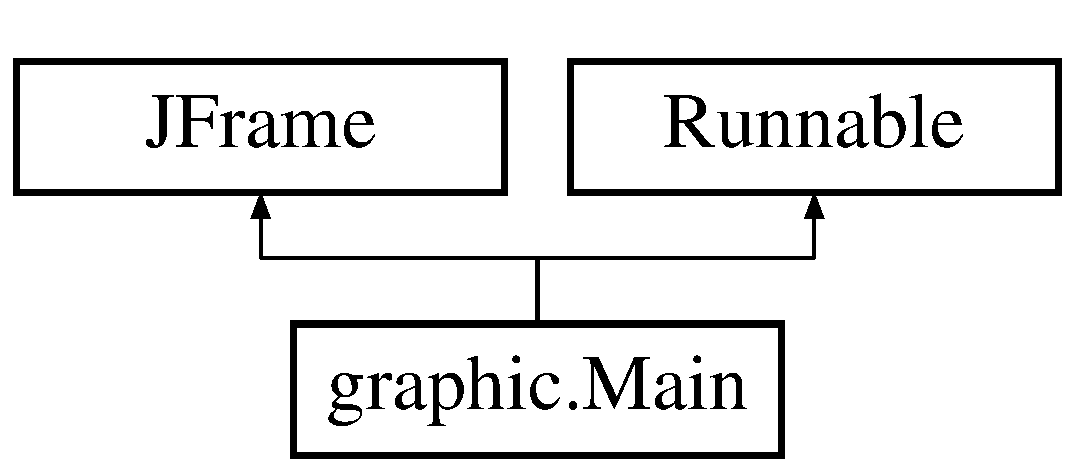
\includegraphics[height=2.000000cm]{classgraphic_1_1_main}
\end{center}
\end{figure}
\subsection*{Public Member Functions}
\begin{DoxyCompactItemize}
\item 
\hyperlink{classgraphic_1_1_main_accc0905da50b389894edb0d06c74d729}{Main} (\hyperlink{classmain_1_1_main}{main.\+Main} main)
\item 
void \hyperlink{classgraphic_1_1_main_a0d2917dabb35ec2691d660a20a663139}{run} ()
\item 
\hyperlink{classmain_1_1_main}{main.\+Main} \hyperlink{classgraphic_1_1_main_a301b089a02920c585b50d06ff024b145}{get\+Main} ()
\item 
void \hyperlink{classgraphic_1_1_main_ad5a607609bf30c7d09d3340c118b4c57}{set\+Main} (\hyperlink{classmain_1_1_main}{main.\+Main} main)
\item 
void \hyperlink{classgraphic_1_1_main_a4c7ddcd2bfc33ac56722e7f6970afbc2}{set\+Energy} (String s)
\end{DoxyCompactItemize}
\subsection*{Public Attributes}
\begin{DoxyCompactItemize}
\item 
javax.\+swing.\+J\+Label \hyperlink{classgraphic_1_1_main_a07b285e66d82f1f90d94a7c61ad939a1}{energy}
\item 
\hypertarget{classgraphic_1_1_main_ac3aa555569610334ab1babed0b83b5c7}{}\label{classgraphic_1_1_main_ac3aa555569610334ab1babed0b83b5c7} 
\hyperlink{classgraphic_1_1_grid_panel}{graphic.\+Grid\+Panel} {\bfseries view}
\end{DoxyCompactItemize}


\subsection{Detailed Description}
Classe principale de l\textquotesingle{}interface graphique. Elle permet d\textquotesingle{}initialiser la grille et d\textquotesingle{}ajouter les éléments graphiques utilisable par les utilisateurs. \begin{DoxyAuthor}{Author}
Maxime 
\end{DoxyAuthor}


\subsection{Constructor \& Destructor Documentation}
\hypertarget{classgraphic_1_1_main_accc0905da50b389894edb0d06c74d729}{}\label{classgraphic_1_1_main_accc0905da50b389894edb0d06c74d729} 
\index{graphic\+::\+Main@{graphic\+::\+Main}!Main@{Main}}
\index{Main@{Main}!graphic\+::\+Main@{graphic\+::\+Main}}
\subsubsection{\texorpdfstring{Main()}{Main()}}
{\footnotesize\ttfamily graphic.\+Main.\+Main (\begin{DoxyParamCaption}\item[{\hyperlink{classmain_1_1_main}{main.\+Main}}]{main }\end{DoxyParamCaption})}

Constructeur de la classe qui permet d\textquotesingle{}initialiser la variable main 
\begin{DoxyParams}{Parameters}
{\em main} & Classe principale du projet \\
\hline
\end{DoxyParams}


\subsection{Member Function Documentation}
\hypertarget{classgraphic_1_1_main_a301b089a02920c585b50d06ff024b145}{}\label{classgraphic_1_1_main_a301b089a02920c585b50d06ff024b145} 
\index{graphic\+::\+Main@{graphic\+::\+Main}!get\+Main@{get\+Main}}
\index{get\+Main@{get\+Main}!graphic\+::\+Main@{graphic\+::\+Main}}
\subsubsection{\texorpdfstring{get\+Main()}{getMain()}}
{\footnotesize\ttfamily \hyperlink{classmain_1_1_main}{main.\+Main} graphic.\+Main.\+get\+Main (\begin{DoxyParamCaption}{ }\end{DoxyParamCaption})}

Getter du main \begin{DoxyReturn}{Returns}
the main 
\end{DoxyReturn}
\hypertarget{classgraphic_1_1_main_a0d2917dabb35ec2691d660a20a663139}{}\label{classgraphic_1_1_main_a0d2917dabb35ec2691d660a20a663139} 
\index{graphic\+::\+Main@{graphic\+::\+Main}!run@{run}}
\index{run@{run}!graphic\+::\+Main@{graphic\+::\+Main}}
\subsubsection{\texorpdfstring{run()}{run()}}
{\footnotesize\ttfamily void graphic.\+Main.\+run (\begin{DoxyParamCaption}{ }\end{DoxyParamCaption})}

Méthode qui permet d\textquotesingle{}initialiser tous les composants graphiques ainsi que d\textquotesingle{}initialiser la grille et ses cellules \hypertarget{classgraphic_1_1_main_a4c7ddcd2bfc33ac56722e7f6970afbc2}{}\label{classgraphic_1_1_main_a4c7ddcd2bfc33ac56722e7f6970afbc2} 
\index{graphic\+::\+Main@{graphic\+::\+Main}!set\+Energy@{set\+Energy}}
\index{set\+Energy@{set\+Energy}!graphic\+::\+Main@{graphic\+::\+Main}}
\subsubsection{\texorpdfstring{set\+Energy()}{setEnergy()}}
{\footnotesize\ttfamily void graphic.\+Main.\+set\+Energy (\begin{DoxyParamCaption}\item[{String}]{s }\end{DoxyParamCaption})}

Setter de l\textquotesingle{}energie permet de modifer le champs de l\textquotesingle{}énergie 
\begin{DoxyParams}{Parameters}
{\em s} & représente la valeur \\
\hline
\end{DoxyParams}
\hypertarget{classgraphic_1_1_main_ad5a607609bf30c7d09d3340c118b4c57}{}\label{classgraphic_1_1_main_ad5a607609bf30c7d09d3340c118b4c57} 
\index{graphic\+::\+Main@{graphic\+::\+Main}!set\+Main@{set\+Main}}
\index{set\+Main@{set\+Main}!graphic\+::\+Main@{graphic\+::\+Main}}
\subsubsection{\texorpdfstring{set\+Main()}{setMain()}}
{\footnotesize\ttfamily void graphic.\+Main.\+set\+Main (\begin{DoxyParamCaption}\item[{\hyperlink{classmain_1_1_main}{main.\+Main}}]{main }\end{DoxyParamCaption})}

Setter du main 
\begin{DoxyParams}{Parameters}
{\em main} & the main to set \\
\hline
\end{DoxyParams}


\subsection{Member Data Documentation}
\hypertarget{classgraphic_1_1_main_a07b285e66d82f1f90d94a7c61ad939a1}{}\label{classgraphic_1_1_main_a07b285e66d82f1f90d94a7c61ad939a1} 
\index{graphic\+::\+Main@{graphic\+::\+Main}!energy@{energy}}
\index{energy@{energy}!graphic\+::\+Main@{graphic\+::\+Main}}
\subsubsection{\texorpdfstring{energy}{energy}}
{\footnotesize\ttfamily javax.\+swing.\+J\+Label graphic.\+Main.\+energy}


\begin{DoxyParams}{Parameters}
{\em args} & the command line arguments energy = label texte qui affiche l\textquotesingle{}énergie dépensée label\+Dust = label qui affiche le texte \char`\"{}\char`\"{} label\+Energy = label qui affiche le texte \char`\"{}\char`\"{} label\+Jewel = label qui affiche le texte \char`\"{}\char`\"{} slider\+Dust = slider de la probabilité d\textquotesingle{}avoir une poussière slider\+Jewel = slider de la probabilité d\textquotesingle{}avoir un bijou slider\+Time = slider de la fréquence d\textquotesingle{}apparition d\textquotesingle{}un item text\+Field\+Dust = champs texte qui affiche la probabilité d\textquotesingle{}avoir une poussière text\+Field\+Jewel = champs texte qui affiche la probabilité d\textquotesingle{}avoir un bijou text\+Field\+Dust = champs texte qui affiche la fréquence d\textquotesingle{}apparition d\textquotesingle{}un item view = la grille qui va recevoir l\textquotesingle{}affichage des items \\
\hline
\end{DoxyParams}


The documentation for this class was generated from the following file\+:\begin{DoxyCompactItemize}
\item 
graphic/Main.\+java\end{DoxyCompactItemize}

\hypertarget{classmain_1_1_main}{}\section{main.\+Main Class Reference}
\label{classmain_1_1_main}\index{main.\+Main@{main.\+Main}}
\subsection*{Public Member Functions}
\begin{DoxyCompactItemize}
\item 
\hyperlink{classmain_1_1_main_a3bd36c15a333d7b594eb71f68a938492}{Main} ()
\item 
\hyperlink{classenvironnement_1_1_environnement}{Environnement} \hyperlink{classmain_1_1_main_a701386aa685b5e10807def95e010d915}{get\+Environnement} ()
\item 
void \hyperlink{classmain_1_1_main_aaf5877a75af1ae2d8f6e35ce6d624301}{set\+Environnement} (\hyperlink{classenvironnement_1_1_environnement}{Environnement} a\+Environnement)
\item 
void \hyperlink{classmain_1_1_main_a79f1b4e1ccb0a641c1d36973af32eca1}{bot\+Move} (\hyperlink{enum_i_a_1_1_direction}{Direction} dir)
\item 
boolean \hyperlink{classmain_1_1_main_a791b90bdd63a0a13054f10b7f4b4e27f}{get\+Dust\+State} ()
\item 
boolean \hyperlink{classmain_1_1_main_aa0df4a294d402074303f47f1fd33a766}{get\+Jewel\+State} ()
\item 
void \hyperlink{classmain_1_1_main_a95439ee2c099d18cc32c6ffd785540ab}{suck} ()
\item 
void \hyperlink{classmain_1_1_main_a007a1feb59e43e37f32b6d8625664986}{pick} ()
\item 
void \hyperlink{classmain_1_1_main_a07fa4830b941140965687c3a2dc8c2e9}{add\+Dust} (int r, int c)
\item 
void \hyperlink{classmain_1_1_main_aaa7affd0b1ef80da03008902969da99b}{add\+Jewel} (int r, int c)
\item 
\hyperlink{classgraphic_1_1_main}{graphic.\+Main} \hyperlink{classmain_1_1_main_a1daa1d9376ab5764f820ee594ff537ce}{get\+Graph} ()
\item 
void \hyperlink{classmain_1_1_main_ab5524b1612bb914ee34f0f0c6cc89a5f}{set\+Graph} (\hyperlink{classgraphic_1_1_main}{graphic.\+Main} graph)
\item 
void \hyperlink{classmain_1_1_main_a3cec64baca52714fb67467ec5d793249}{set\+Frequency} (int freq)
\item 
void \hyperlink{classmain_1_1_main_a4fe27a92bfb4ab6b91100b78d5e60984}{set\+Dust\+Prob} (int prob)
\item 
void \hyperlink{classmain_1_1_main_a300ba85da3a72bc7ca9ad5f5b5a104ed}{set\+Jewel\+Prob} (int prob)
\item 
boolean \hyperlink{classmain_1_1_main_a5052a776c99a2dadce1fe83501e5860e}{is\+Cell\+Enabled} (\hyperlink{classenvironnement_1_1_cell}{Cell} c)
\item 
\hyperlink{class_i_a_1_1_bender}{Bender} \hyperlink{classmain_1_1_main_afa1c1d8de2dbeb639cf157413f82aec2}{get\+Robot} ()
\item 
void \hyperlink{classmain_1_1_main_ab2bea62d3409f687309c3ce697825c63}{set\+Robot} (\hyperlink{class_i_a_1_1_bender}{Bender} robot)
\item 
void \hyperlink{classmain_1_1_main_a676892cd2586d3b8d20e05451f306fba}{update\+Conso} (int i)
\end{DoxyCompactItemize}
\subsection*{Static Public Member Functions}
\begin{DoxyCompactItemize}
\item 
static void \hyperlink{classmain_1_1_main_ab607ced846a257d28e8f81d1820d587c}{main} (String \mbox{[}$\,$\mbox{]} args)
\end{DoxyCompactItemize}


\subsection{Detailed Description}
Classe principale du programme Lance les autres modules (Environnement, Robot et Graphique) et joue le rôle d\textquotesingle{}interface \begin{DoxyAuthor}{Author}
Thomas 
\end{DoxyAuthor}


\subsection{Constructor \& Destructor Documentation}
\hypertarget{classmain_1_1_main_a3bd36c15a333d7b594eb71f68a938492}{}\label{classmain_1_1_main_a3bd36c15a333d7b594eb71f68a938492} 
\index{main\+::\+Main@{main\+::\+Main}!Main@{Main}}
\index{Main@{Main}!main\+::\+Main@{main\+::\+Main}}
\subsubsection{\texorpdfstring{Main()}{Main()}}
{\footnotesize\ttfamily main.\+Main.\+Main (\begin{DoxyParamCaption}{ }\end{DoxyParamCaption})}

Constructeur de la classe Lance tous les modules dans des threads distincts 

\subsection{Member Function Documentation}
\hypertarget{classmain_1_1_main_a07fa4830b941140965687c3a2dc8c2e9}{}\label{classmain_1_1_main_a07fa4830b941140965687c3a2dc8c2e9} 
\index{main\+::\+Main@{main\+::\+Main}!add\+Dust@{add\+Dust}}
\index{add\+Dust@{add\+Dust}!main\+::\+Main@{main\+::\+Main}}
\subsubsection{\texorpdfstring{add\+Dust()}{addDust()}}
{\footnotesize\ttfamily void main.\+Main.\+add\+Dust (\begin{DoxyParamCaption}\item[{int}]{r,  }\item[{int}]{c }\end{DoxyParamCaption})}

Méthode appelée par l\textquotesingle{}interface graphique ou l\textquotesingle{}environnement, cet appel est déterminé par \hyperlink{}{Stack\+Trace\+Element} Ajoute de la poussière soit à l\textquotesingle{}environnement soit à l\textquotesingle{}interface graphique dépendamment de l\textquotesingle{}appelant 
\begin{DoxyParams}{Parameters}
{\em r} & La ligne de la cellule où ajouter de la poussière \\
\hline
{\em c} & La colonne de la cellule où ajouter de la poussière \\
\hline
\end{DoxyParams}
\hypertarget{classmain_1_1_main_aaa7affd0b1ef80da03008902969da99b}{}\label{classmain_1_1_main_aaa7affd0b1ef80da03008902969da99b} 
\index{main\+::\+Main@{main\+::\+Main}!add\+Jewel@{add\+Jewel}}
\index{add\+Jewel@{add\+Jewel}!main\+::\+Main@{main\+::\+Main}}
\subsubsection{\texorpdfstring{add\+Jewel()}{addJewel()}}
{\footnotesize\ttfamily void main.\+Main.\+add\+Jewel (\begin{DoxyParamCaption}\item[{int}]{r,  }\item[{int}]{c }\end{DoxyParamCaption})}

Méthode appelée par l\textquotesingle{}interface graphique ou l\textquotesingle{}environnement, cet appel est déterminé par \hyperlink{}{Stack\+Trace\+Element} Ajoute un bijou soit à l\textquotesingle{}environnement soit à l\textquotesingle{}interface graphique dépendamment de l\textquotesingle{}appelant 
\begin{DoxyParams}{Parameters}
{\em r} & La ligne de la cellule où ajouter un bijou \\
\hline
{\em c} & La colonne de la cellule où ajouter un bijou \\
\hline
\end{DoxyParams}
\hypertarget{classmain_1_1_main_a79f1b4e1ccb0a641c1d36973af32eca1}{}\label{classmain_1_1_main_a79f1b4e1ccb0a641c1d36973af32eca1} 
\index{main\+::\+Main@{main\+::\+Main}!bot\+Move@{bot\+Move}}
\index{bot\+Move@{bot\+Move}!main\+::\+Main@{main\+::\+Main}}
\subsubsection{\texorpdfstring{bot\+Move()}{botMove()}}
{\footnotesize\ttfamily void main.\+Main.\+bot\+Move (\begin{DoxyParamCaption}\item[{\hyperlink{enum_i_a_1_1_direction}{Direction}}]{dir }\end{DoxyParamCaption})}

Méthode appelée lorsque le robot bouge Quelque soit la direction désirée, la méthode vérifie que la cellule demandée existe et est valable 
\begin{DoxyParams}{Parameters}
{\em dir} & La direction dans laquelle le robot bouge \\
\hline
\end{DoxyParams}
\hypertarget{classmain_1_1_main_a791b90bdd63a0a13054f10b7f4b4e27f}{}\label{classmain_1_1_main_a791b90bdd63a0a13054f10b7f4b4e27f} 
\index{main\+::\+Main@{main\+::\+Main}!get\+Dust\+State@{get\+Dust\+State}}
\index{get\+Dust\+State@{get\+Dust\+State}!main\+::\+Main@{main\+::\+Main}}
\subsubsection{\texorpdfstring{get\+Dust\+State()}{getDustState()}}
{\footnotesize\ttfamily boolean main.\+Main.\+get\+Dust\+State (\begin{DoxyParamCaption}{ }\end{DoxyParamCaption})}

Getter de l\textquotesingle{}état de poussière de la cellule courante du robot \begin{DoxyReturn}{Returns}
Si la cellule possède de la poussière 
\end{DoxyReturn}
\hypertarget{classmain_1_1_main_a701386aa685b5e10807def95e010d915}{}\label{classmain_1_1_main_a701386aa685b5e10807def95e010d915} 
\index{main\+::\+Main@{main\+::\+Main}!get\+Environnement@{get\+Environnement}}
\index{get\+Environnement@{get\+Environnement}!main\+::\+Main@{main\+::\+Main}}
\subsubsection{\texorpdfstring{get\+Environnement()}{getEnvironnement()}}
{\footnotesize\ttfamily \hyperlink{classenvironnement_1_1_environnement}{Environnement} main.\+Main.\+get\+Environnement (\begin{DoxyParamCaption}{ }\end{DoxyParamCaption})}

Getter de l\textquotesingle{}environnement \begin{DoxyReturn}{Returns}
L\textquotesingle{}environnement 
\end{DoxyReturn}
\hypertarget{classmain_1_1_main_a1daa1d9376ab5764f820ee594ff537ce}{}\label{classmain_1_1_main_a1daa1d9376ab5764f820ee594ff537ce} 
\index{main\+::\+Main@{main\+::\+Main}!get\+Graph@{get\+Graph}}
\index{get\+Graph@{get\+Graph}!main\+::\+Main@{main\+::\+Main}}
\subsubsection{\texorpdfstring{get\+Graph()}{getGraph()}}
{\footnotesize\ttfamily \hyperlink{classgraphic_1_1_main}{graphic.\+Main} main.\+Main.\+get\+Graph (\begin{DoxyParamCaption}{ }\end{DoxyParamCaption})}

Getter de l\textquotesingle{}interface graphique \begin{DoxyReturn}{Returns}
L\textquotesingle{}interface graphique 
\end{DoxyReturn}
\hypertarget{classmain_1_1_main_aa0df4a294d402074303f47f1fd33a766}{}\label{classmain_1_1_main_aa0df4a294d402074303f47f1fd33a766} 
\index{main\+::\+Main@{main\+::\+Main}!get\+Jewel\+State@{get\+Jewel\+State}}
\index{get\+Jewel\+State@{get\+Jewel\+State}!main\+::\+Main@{main\+::\+Main}}
\subsubsection{\texorpdfstring{get\+Jewel\+State()}{getJewelState()}}
{\footnotesize\ttfamily boolean main.\+Main.\+get\+Jewel\+State (\begin{DoxyParamCaption}{ }\end{DoxyParamCaption})}

Getter de l\textquotesingle{}état de bijou de la cellule courante du robot \begin{DoxyReturn}{Returns}
Si la cellule possède un bijou 
\end{DoxyReturn}
\hypertarget{classmain_1_1_main_afa1c1d8de2dbeb639cf157413f82aec2}{}\label{classmain_1_1_main_afa1c1d8de2dbeb639cf157413f82aec2} 
\index{main\+::\+Main@{main\+::\+Main}!get\+Robot@{get\+Robot}}
\index{get\+Robot@{get\+Robot}!main\+::\+Main@{main\+::\+Main}}
\subsubsection{\texorpdfstring{get\+Robot()}{getRobot()}}
{\footnotesize\ttfamily \hyperlink{class_i_a_1_1_bender}{Bender} main.\+Main.\+get\+Robot (\begin{DoxyParamCaption}{ }\end{DoxyParamCaption})}

Getter pour le robot \begin{DoxyReturn}{Returns}
Le robot 
\end{DoxyReturn}
\hypertarget{classmain_1_1_main_a5052a776c99a2dadce1fe83501e5860e}{}\label{classmain_1_1_main_a5052a776c99a2dadce1fe83501e5860e} 
\index{main\+::\+Main@{main\+::\+Main}!is\+Cell\+Enabled@{is\+Cell\+Enabled}}
\index{is\+Cell\+Enabled@{is\+Cell\+Enabled}!main\+::\+Main@{main\+::\+Main}}
\subsubsection{\texorpdfstring{is\+Cell\+Enabled()}{isCellEnabled()}}
{\footnotesize\ttfamily boolean main.\+Main.\+is\+Cell\+Enabled (\begin{DoxyParamCaption}\item[{\hyperlink{classenvironnement_1_1_cell}{Cell}}]{c }\end{DoxyParamCaption})}

Méthode appelée par le robot pour savoir si une cellule est valable Cette méthode traduit les coordonnées exprimées par le robot en coordonnées réelles pour l\textquotesingle{}environnement 
\begin{DoxyParams}{Parameters}
{\em c} & La cellule souhaitée \\
\hline
\end{DoxyParams}
\begin{DoxyReturn}{Returns}
Si la cellule est valable 
\end{DoxyReturn}
\hypertarget{classmain_1_1_main_ab607ced846a257d28e8f81d1820d587c}{}\label{classmain_1_1_main_ab607ced846a257d28e8f81d1820d587c} 
\index{main\+::\+Main@{main\+::\+Main}!main@{main}}
\index{main@{main}!main\+::\+Main@{main\+::\+Main}}
\subsubsection{\texorpdfstring{main()}{main()}}
{\footnotesize\ttfamily static void main.\+Main.\+main (\begin{DoxyParamCaption}\item[{String \mbox{[}$\,$\mbox{]}}]{args }\end{DoxyParamCaption})\hspace{0.3cm}{\ttfamily [static]}}

Fonction appelée au lancement du programme Construit un \hyperlink{classmain_1_1_main}{Main} ce qui a pour effet de lancer le programme 
\begin{DoxyParams}{Parameters}
{\em args} & Paramètres d\textquotesingle{}appels \\
\hline
\end{DoxyParams}
\hypertarget{classmain_1_1_main_a007a1feb59e43e37f32b6d8625664986}{}\label{classmain_1_1_main_a007a1feb59e43e37f32b6d8625664986} 
\index{main\+::\+Main@{main\+::\+Main}!pick@{pick}}
\index{pick@{pick}!main\+::\+Main@{main\+::\+Main}}
\subsubsection{\texorpdfstring{pick()}{pick()}}
{\footnotesize\ttfamily void main.\+Main.\+pick (\begin{DoxyParamCaption}{ }\end{DoxyParamCaption})}

Le robot prend un bijou présent sur la cellule \hypertarget{classmain_1_1_main_a4fe27a92bfb4ab6b91100b78d5e60984}{}\label{classmain_1_1_main_a4fe27a92bfb4ab6b91100b78d5e60984} 
\index{main\+::\+Main@{main\+::\+Main}!set\+Dust\+Prob@{set\+Dust\+Prob}}
\index{set\+Dust\+Prob@{set\+Dust\+Prob}!main\+::\+Main@{main\+::\+Main}}
\subsubsection{\texorpdfstring{set\+Dust\+Prob()}{setDustProb()}}
{\footnotesize\ttfamily void main.\+Main.\+set\+Dust\+Prob (\begin{DoxyParamCaption}\item[{int}]{prob }\end{DoxyParamCaption})}

Setter de la probabilité d\textquotesingle{}apparition de poussière 
\begin{DoxyParams}{Parameters}
{\em prob} & Nouvelle probabilité d\textquotesingle{}apparition de poussière \\
\hline
\end{DoxyParams}
\hypertarget{classmain_1_1_main_aaf5877a75af1ae2d8f6e35ce6d624301}{}\label{classmain_1_1_main_aaf5877a75af1ae2d8f6e35ce6d624301} 
\index{main\+::\+Main@{main\+::\+Main}!set\+Environnement@{set\+Environnement}}
\index{set\+Environnement@{set\+Environnement}!main\+::\+Main@{main\+::\+Main}}
\subsubsection{\texorpdfstring{set\+Environnement()}{setEnvironnement()}}
{\footnotesize\ttfamily void main.\+Main.\+set\+Environnement (\begin{DoxyParamCaption}\item[{\hyperlink{classenvironnement_1_1_environnement}{Environnement}}]{a\+Environnement }\end{DoxyParamCaption})}

Setter de l\textquotesingle{}environnement 
\begin{DoxyParams}{Parameters}
{\em a\+Environnement} & L\textquotesingle{}environnement \\
\hline
\end{DoxyParams}
\hypertarget{classmain_1_1_main_a3cec64baca52714fb67467ec5d793249}{}\label{classmain_1_1_main_a3cec64baca52714fb67467ec5d793249} 
\index{main\+::\+Main@{main\+::\+Main}!set\+Frequency@{set\+Frequency}}
\index{set\+Frequency@{set\+Frequency}!main\+::\+Main@{main\+::\+Main}}
\subsubsection{\texorpdfstring{set\+Frequency()}{setFrequency()}}
{\footnotesize\ttfamily void main.\+Main.\+set\+Frequency (\begin{DoxyParamCaption}\item[{int}]{freq }\end{DoxyParamCaption})}

Setter du temps inter boucle pour les générations de poussière et de bijoux 
\begin{DoxyParams}{Parameters}
{\em freq} & Le nouveau temps inter boucle \\
\hline
\end{DoxyParams}
\hypertarget{classmain_1_1_main_ab5524b1612bb914ee34f0f0c6cc89a5f}{}\label{classmain_1_1_main_ab5524b1612bb914ee34f0f0c6cc89a5f} 
\index{main\+::\+Main@{main\+::\+Main}!set\+Graph@{set\+Graph}}
\index{set\+Graph@{set\+Graph}!main\+::\+Main@{main\+::\+Main}}
\subsubsection{\texorpdfstring{set\+Graph()}{setGraph()}}
{\footnotesize\ttfamily void main.\+Main.\+set\+Graph (\begin{DoxyParamCaption}\item[{\hyperlink{classgraphic_1_1_main}{graphic.\+Main}}]{graph }\end{DoxyParamCaption})}

Setter de l\textquotesingle{}interface graphique 
\begin{DoxyParams}{Parameters}
{\em graph} & L\textquotesingle{}interface graphique \\
\hline
\end{DoxyParams}
\hypertarget{classmain_1_1_main_a300ba85da3a72bc7ca9ad5f5b5a104ed}{}\label{classmain_1_1_main_a300ba85da3a72bc7ca9ad5f5b5a104ed} 
\index{main\+::\+Main@{main\+::\+Main}!set\+Jewel\+Prob@{set\+Jewel\+Prob}}
\index{set\+Jewel\+Prob@{set\+Jewel\+Prob}!main\+::\+Main@{main\+::\+Main}}
\subsubsection{\texorpdfstring{set\+Jewel\+Prob()}{setJewelProb()}}
{\footnotesize\ttfamily void main.\+Main.\+set\+Jewel\+Prob (\begin{DoxyParamCaption}\item[{int}]{prob }\end{DoxyParamCaption})}

Setter de la probabilité d\textquotesingle{}apparition de bijoux 
\begin{DoxyParams}{Parameters}
{\em prob} & Nouvelle probabilité d\textquotesingle{}apparition de bijoux \\
\hline
\end{DoxyParams}
\hypertarget{classmain_1_1_main_ab2bea62d3409f687309c3ce697825c63}{}\label{classmain_1_1_main_ab2bea62d3409f687309c3ce697825c63} 
\index{main\+::\+Main@{main\+::\+Main}!set\+Robot@{set\+Robot}}
\index{set\+Robot@{set\+Robot}!main\+::\+Main@{main\+::\+Main}}
\subsubsection{\texorpdfstring{set\+Robot()}{setRobot()}}
{\footnotesize\ttfamily void main.\+Main.\+set\+Robot (\begin{DoxyParamCaption}\item[{\hyperlink{class_i_a_1_1_bender}{Bender}}]{robot }\end{DoxyParamCaption})}

Setter pour le robot 
\begin{DoxyParams}{Parameters}
{\em robot} & Le robot \\
\hline
\end{DoxyParams}
\hypertarget{classmain_1_1_main_a95439ee2c099d18cc32c6ffd785540ab}{}\label{classmain_1_1_main_a95439ee2c099d18cc32c6ffd785540ab} 
\index{main\+::\+Main@{main\+::\+Main}!suck@{suck}}
\index{suck@{suck}!main\+::\+Main@{main\+::\+Main}}
\subsubsection{\texorpdfstring{suck()}{suck()}}
{\footnotesize\ttfamily void main.\+Main.\+suck (\begin{DoxyParamCaption}{ }\end{DoxyParamCaption})}

Le robot aspire tous les objets présents sur la cellule courante \hypertarget{classmain_1_1_main_a676892cd2586d3b8d20e05451f306fba}{}\label{classmain_1_1_main_a676892cd2586d3b8d20e05451f306fba} 
\index{main\+::\+Main@{main\+::\+Main}!update\+Conso@{update\+Conso}}
\index{update\+Conso@{update\+Conso}!main\+::\+Main@{main\+::\+Main}}
\subsubsection{\texorpdfstring{update\+Conso()}{updateConso()}}
{\footnotesize\ttfamily void main.\+Main.\+update\+Conso (\begin{DoxyParamCaption}\item[{int}]{i }\end{DoxyParamCaption})}

Méthode appelée par le robot pour mettre à jour le niveau d\textquotesingle{}énergie consommé dans l\textquotesingle{}interface graphique 
\begin{DoxyParams}{Parameters}
{\em i} & Nouvelle valeur de la consommation en énergie \\
\hline
\end{DoxyParams}


The documentation for this class was generated from the following file\+:\begin{DoxyCompactItemize}
\item 
main/Main.\+java\end{DoxyCompactItemize}

\hypertarget{classenvironnement_1_1_object}{}\section{environnement.\+Object Class Reference}
\label{classenvironnement_1_1_object}\index{environnement.\+Object@{environnement.\+Object}}
\subsection*{Public Member Functions}
\begin{DoxyCompactItemize}
\item 
\hyperlink{classenvironnement_1_1_object_a1e78f61fea8a24042861aca518768958}{Object} (\hyperlink{enumenvironnement_1_1_type}{Type} t)
\item 
\hyperlink{enumenvironnement_1_1_type}{Type} \hyperlink{classenvironnement_1_1_object_a12c1066fd1d4b8a10d5a982decc2142f}{get\+Type} ()
\item 
void \hyperlink{classenvironnement_1_1_object_aa761d751ee5d7549420d99ffa08ec378}{set\+Type} (\hyperlink{enumenvironnement_1_1_type}{Type} type)
\end{DoxyCompactItemize}


\subsection{Detailed Description}
Classe représentant un objet présent sur une cellule Cette classe a été implementée dans l\textquotesingle{}optique d\textquotesingle{}ajouter des contraintes sur ces objets telles que le poids Cette fonctionnalité n\textquotesingle{}a pas encore été développée. \begin{DoxyAuthor}{Author}
Thomas 
\end{DoxyAuthor}


\subsection{Constructor \& Destructor Documentation}
\hypertarget{classenvironnement_1_1_object_a1e78f61fea8a24042861aca518768958}{}\label{classenvironnement_1_1_object_a1e78f61fea8a24042861aca518768958} 
\index{environnement\+::\+Object@{environnement\+::\+Object}!Object@{Object}}
\index{Object@{Object}!environnement\+::\+Object@{environnement\+::\+Object}}
\subsubsection{\texorpdfstring{Object()}{Object()}}
{\footnotesize\ttfamily environnement.\+Object.\+Object (\begin{DoxyParamCaption}\item[{\hyperlink{enumenvironnement_1_1_type}{Type}}]{t }\end{DoxyParamCaption})}

Constructeur de la classe 
\begin{DoxyParams}{Parameters}
{\em t} & \hyperlink{enumenvironnement_1_1_type}{Type} de l\textquotesingle{}objet \\
\hline
\end{DoxyParams}


\subsection{Member Function Documentation}
\hypertarget{classenvironnement_1_1_object_a12c1066fd1d4b8a10d5a982decc2142f}{}\label{classenvironnement_1_1_object_a12c1066fd1d4b8a10d5a982decc2142f} 
\index{environnement\+::\+Object@{environnement\+::\+Object}!get\+Type@{get\+Type}}
\index{get\+Type@{get\+Type}!environnement\+::\+Object@{environnement\+::\+Object}}
\subsubsection{\texorpdfstring{get\+Type()}{getType()}}
{\footnotesize\ttfamily \hyperlink{enumenvironnement_1_1_type}{Type} environnement.\+Object.\+get\+Type (\begin{DoxyParamCaption}{ }\end{DoxyParamCaption})}

Getter du type de l\textquotesingle{}objet \begin{DoxyReturn}{Returns}
Le type de l\textquotesingle{}objet 
\end{DoxyReturn}
\hypertarget{classenvironnement_1_1_object_aa761d751ee5d7549420d99ffa08ec378}{}\label{classenvironnement_1_1_object_aa761d751ee5d7549420d99ffa08ec378} 
\index{environnement\+::\+Object@{environnement\+::\+Object}!set\+Type@{set\+Type}}
\index{set\+Type@{set\+Type}!environnement\+::\+Object@{environnement\+::\+Object}}
\subsubsection{\texorpdfstring{set\+Type()}{setType()}}
{\footnotesize\ttfamily void environnement.\+Object.\+set\+Type (\begin{DoxyParamCaption}\item[{\hyperlink{enumenvironnement_1_1_type}{Type}}]{type }\end{DoxyParamCaption})}

Setter du type de l\textquotesingle{}objet 
\begin{DoxyParams}{Parameters}
{\em type} & Le type de l\textquotesingle{}objet \\
\hline
\end{DoxyParams}


The documentation for this class was generated from the following file\+:\begin{DoxyCompactItemize}
\item 
environnement/Object.\+java\end{DoxyCompactItemize}

\hypertarget{classgraphic_1_1_popup_menu}{}\section{graphic.\+Popup\+Menu Class Reference}
\label{classgraphic_1_1_popup_menu}\index{graphic.\+Popup\+Menu@{graphic.\+Popup\+Menu}}
Inheritance diagram for graphic.\+Popup\+Menu\+:\begin{figure}[H]
\begin{center}
\leavevmode
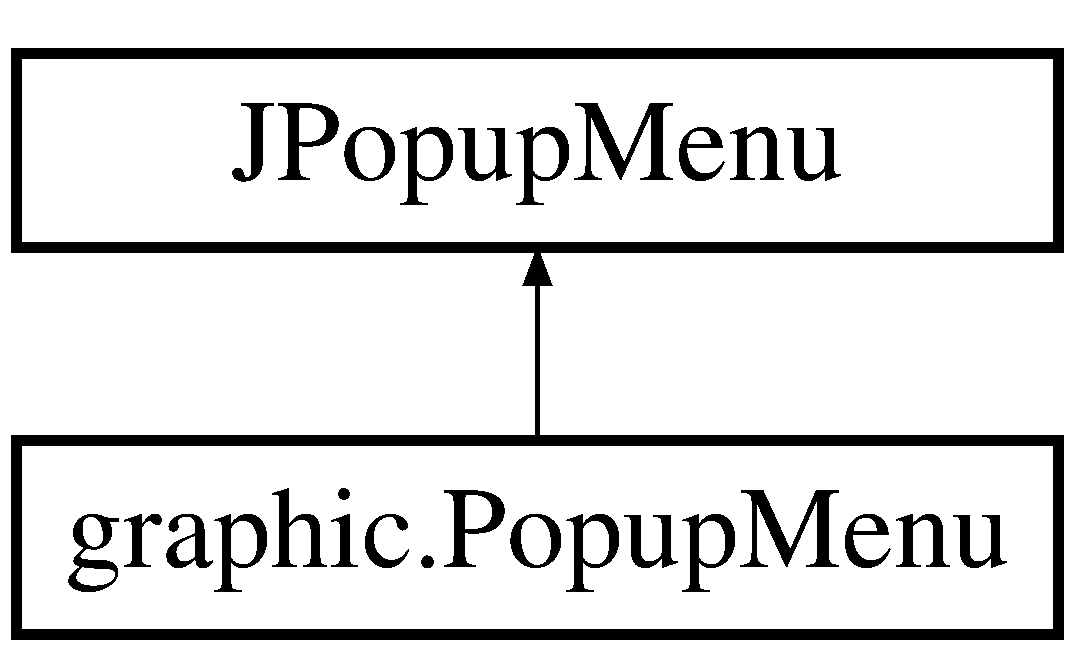
\includegraphics[height=2.000000cm]{classgraphic_1_1_popup_menu}
\end{center}
\end{figure}
\subsection*{Public Member Functions}
\begin{DoxyCompactItemize}
\item 
\hyperlink{classgraphic_1_1_popup_menu_ae43d83c623d5066793d503539ea209e6}{Popup\+Menu} (\hyperlink{classgraphic_1_1_cell_pane}{Cell\+Pane} c)
\end{DoxyCompactItemize}


\subsection{Detailed Description}
Classe qui représente le menu contextuel d\textquotesingle{}une cellule \begin{DoxyAuthor}{Author}
Maxime 
\end{DoxyAuthor}


\subsection{Constructor \& Destructor Documentation}
\hypertarget{classgraphic_1_1_popup_menu_ae43d83c623d5066793d503539ea209e6}{}\label{classgraphic_1_1_popup_menu_ae43d83c623d5066793d503539ea209e6} 
\index{graphic\+::\+Popup\+Menu@{graphic\+::\+Popup\+Menu}!Popup\+Menu@{Popup\+Menu}}
\index{Popup\+Menu@{Popup\+Menu}!graphic\+::\+Popup\+Menu@{graphic\+::\+Popup\+Menu}}
\subsubsection{\texorpdfstring{Popup\+Menu()}{PopupMenu()}}
{\footnotesize\ttfamily graphic.\+Popup\+Menu.\+Popup\+Menu (\begin{DoxyParamCaption}\item[{\hyperlink{classgraphic_1_1_cell_pane}{Cell\+Pane}}]{c }\end{DoxyParamCaption})}

Constructeur de la classe qui permet d\textquotesingle{}initialiser le menu ainsi que les listeneners 
\begin{DoxyParams}{Parameters}
{\em c} & = la cellule mère \\
\hline
\end{DoxyParams}


The documentation for this class was generated from the following file\+:\begin{DoxyCompactItemize}
\item 
graphic/Popup\+Menu.\+java\end{DoxyCompactItemize}

\hypertarget{enumenvironnement_1_1_type}{}\section{environnement.\+Type Enum Reference}
\label{enumenvironnement_1_1_type}\index{environnement.\+Type@{environnement.\+Type}}
\subsection*{Public Attributes}
\begin{DoxyCompactItemize}
\item 
\hyperlink{enumenvironnement_1_1_type_a1e69fa75f3320089da9616bcbd4c213f}{D\+U\+ST}
\item 
\hyperlink{enumenvironnement_1_1_type_a3bbca3efc63d402d324b7a3fa7f5e892}{J\+E\+W\+EL}
\end{DoxyCompactItemize}


\subsection{Detailed Description}
Enum des types possible d\textquotesingle{}objet \begin{DoxyAuthor}{Author}
Thomas 
\end{DoxyAuthor}


\subsection{Member Data Documentation}
\hypertarget{enumenvironnement_1_1_type_a1e69fa75f3320089da9616bcbd4c213f}{}\label{enumenvironnement_1_1_type_a1e69fa75f3320089da9616bcbd4c213f} 
\index{environnement\+::\+Type@{environnement\+::\+Type}!D\+U\+ST@{D\+U\+ST}}
\index{D\+U\+ST@{D\+U\+ST}!environnement\+::\+Type@{environnement\+::\+Type}}
\subsubsection{\texorpdfstring{D\+U\+ST}{DUST}}
{\footnotesize\ttfamily environnement.\+Type.\+D\+U\+ST}

Correspond à une poussière \hypertarget{enumenvironnement_1_1_type_a3bbca3efc63d402d324b7a3fa7f5e892}{}\label{enumenvironnement_1_1_type_a3bbca3efc63d402d324b7a3fa7f5e892} 
\index{environnement\+::\+Type@{environnement\+::\+Type}!J\+E\+W\+EL@{J\+E\+W\+EL}}
\index{J\+E\+W\+EL@{J\+E\+W\+EL}!environnement\+::\+Type@{environnement\+::\+Type}}
\subsubsection{\texorpdfstring{J\+E\+W\+EL}{JEWEL}}
{\footnotesize\ttfamily environnement.\+Type.\+J\+E\+W\+EL}

Correspond à un bijou 

The documentation for this enum was generated from the following file\+:\begin{DoxyCompactItemize}
\item 
environnement/Type.\+java\end{DoxyCompactItemize}

%--- End generated contents ---

% Index
\backmatter
\newpage
\phantomsection
\clearemptydoublepage
\addcontentsline{toc}{chapter}{Index}
\printindex

\end{document}
